% ML-Based Leakage Current Estimation for Static CMOS -- course project report (D10).
% Compiled on Overleaf (pdfLaTeX): upload report/overleaf.zip, see README.md.
% Every number comes from generated/numbers.tex and generated/tab_*.tex (report/make_numbers.py).

\documentclass[11pt,a4paper]{article}

\usepackage[margin=2.5cm]{geometry}
\usepackage[T1]{fontenc}   % proper glyphs for _ < > | in \texttt and generated text
\usepackage{lmodern}
\usepackage{amsmath}
\usepackage{array}         % >{...}p{...} columns in tables
\usepackage{booktabs}
\usepackage{graphicx}
\usepackage{float}
\usepackage{xcolor}
\usepackage{caption}
\usepackage{siunitx}       % v3 (\qty) -- default on Overleaf
\usepackage{hyperref}      % load last

\graphicspath{{figures/}}
\captionsetup{font=small, labelfont=bf}
\sisetup{exponent-product = \times}
\hypersetup{colorlinks=true, linkcolor=blue!50!black, urlcolor=blue!50!black,
            citecolor=blue!50!black}

% Placeholder for text still to be written (also used by generated/numbers.tex for
% missing inputs). Search the PDF for "TODO" before submitting.
\newcommand{\todo}[1]{\textcolor{red}{\textbf{[TODO: #1]}}}

% Shrink a (generated) table to the text width only if it is wider; graphicx only.
\newsavebox{\fitbox}
\newcommand{\fittable}[1]{%
  \sbox{\fitbox}{#1}%
  \ifdim\wd\fitbox>\linewidth\resizebox{\linewidth}{!}{\usebox{\fitbox}}\else\usebox{\fitbox}\fi}

% Generated by report/make_numbers.py. Do not edit: rerun the script after `make all`.
% Sources: results/tables/*.csv, artifacts/env.json, configs/project.yaml, data/*.csv

\newcommand{\TeamName}{Hot Hot Chips}
\newcommand{\TechNode}{32nm\_LP}
\newcommand{\ModelFile}{\texttt{pdk/32nm\_LP.pm}}
\newcommand{\VDDnom}{\qty{0.9}{\volt}}
\newcommand{\VDDtol}{\qty{10}{\percent}}
\newcommand{\VDDmin}{\qty{0.81}{\volt}}
\newcommand{\VDDmax}{\qty{0.99}{\volt}}
\newcommand{\Lmin}{\qty{32}{\nano\metre}}
\newcommand{\TestCircuit}{8-bit parity checker}
\newcommand{\TestCircuitKey}{\texttt{parity8}}
\newcommand{\TempMin}{\qty{-40}{\degreeCelsius}}
\newcommand{\TempMax}{\qty{125}{\degreeCelsius}}
\newcommand{\WMultMin}{1}
\newcommand{\WMultMax}{8}
\newcommand{\ProcessTol}{\qty{10}{\percent}}
\newcommand{\NmosWMult}{2}
\newcommand{\PmosWMult}{4}
\newcommand{\NumCorners}{\num{200}}
\newcommand{\IFloor}{\qty{1e-15}{\ampere}}
\newcommand{\SplitScheme}{70/15/15}
\newcommand{\SeedTransistorData}{1001}
\newcommand{\SeedSplit}{42}
\newcommand{\SeedTraining}{7}
\newcommand{\SeedCorners}{2026}
\newcommand{\SelectionMetric}{\texttt{p95\_err\_pct}}
\newcommand{\SimVersion}{ngspice-47}
\newcommand{\PythonVersion}{3.12.15}
\newcommand{\VerNumpy}{2.5.4}
\newcommand{\VerPandas}{3.1.0}
\newcommand{\VerScikitLearn}{1.9.1}
\newcommand{\VerLightgbm}{4.7.0}
\newcommand{\EnvCommit}{\texttt{de703eb}}
\newcommand{\EnvDate}{2026-11-15}
\newcommand{\RowsPerCase}{\num{30000}}
\newcommand{\NTrain}{\num{21000}}
\newcommand{\NVal}{\num{4500}}
\newcommand{\NTest}{\num{4500}}
\newcommand{\NumGateSims}{\num{3600}}
\newcommand{\KirchhoffMaxAbsNmosOn}{\qty{9.7e-15}{\ampere}}
\newcommand{\KirchhoffMaxRelNmosOn}{\num{3.7e-08}}
\newcommand{\KirchhoffMaxAbsNmosOff}{\qty{9.9e-21}{\ampere}}
\newcommand{\KirchhoffMaxRelNmosOff}{\num{1.1e-10}}
\newcommand{\KirchhoffMaxAbsPmosOn}{\qty{8.8e-15}{\ampere}}
\newcommand{\KirchhoffMaxRelPmosOn}{\num{1.3e-02}}
\newcommand{\KirchhoffMaxAbsPmosOff}{\qty{1.7e-16}{\ampere}}
\newcommand{\KirchhoffMaxRelPmosOff}{\num{8.5e-02}}
\newcommand{\KirchhoffMedianAbsNmosOn}{\qty{3.4e-21}{\ampere}}
\newcommand{\KirchhoffPninetyfiveAbsNmosOn}{\qty{3.6e-16}{\ampere}}
\newcommand{\KirchhoffMedianRelNmosOn}{\num{1.1e-11}}
\newcommand{\KirchhoffPninetyfiveRelNmosOn}{\num{1.4e-10}}
\newcommand{\KirchhoffMedianAbsNmosOff}{\qty{1.1e-24}{\ampere}}
\newcommand{\KirchhoffPninetyfiveAbsNmosOff}{\qty{4.8e-22}{\ampere}}
\newcommand{\KirchhoffMedianRelNmosOff}{\num{1.2e-11}}
\newcommand{\KirchhoffPninetyfiveRelNmosOff}{\num{5.9e-11}}
\newcommand{\KirchhoffMedianAbsPmosOn}{\qty{3.1e-17}{\ampere}}
\newcommand{\KirchhoffPninetyfiveAbsPmosOn}{\qty{2.0e-16}{\ampere}}
\newcommand{\KirchhoffMedianRelPmosOn}{\num{1.3e-07}}
\newcommand{\KirchhoffPninetyfiveRelPmosOn}{\num{3.5e-03}}
\newcommand{\KirchhoffMedianAbsPmosOff}{\qty{2.6e-17}{\ampere}}
\newcommand{\KirchhoffPninetyfiveAbsPmosOff}{\qty{7.2e-17}{\ampere}}
\newcommand{\KirchhoffMedianRelPmosOff}{\num{1.5e-04}}
\newcommand{\KirchhoffPninetyfiveRelPmosOff}{\num{4.7e-03}}
\newcommand{\KirchhoffWorstRel}{\num{8.5e-02}}
\newcommand{\KirchhoffWorstAbs}{\qty{9.7e-15}{\ampere}}
\newcommand{\ChosenModelNmosOn}{GBDT}
\newcommand{\ValMedianErrNmosOn}{\qty{5.0}{\percent}}
\newcommand{\ValPninetyfiveErrNmosOn}{\qty{47.3}{\percent}}
\newcommand{\TestMedianErrNmosOnId}{\qty{9.00}{\percent}}
\newcommand{\TestPninetyfiveErrNmosOnId}{\qty{91.1}{\percent}}
\newcommand{\TestRtwoNmosOnId}{\num{0.9566}}
\newcommand{\TestMeanAccNmosOnId}{\qty{65.2}{\percent}}
\newcommand{\TestMedianErrNmosOnIg}{\qty{2.90}{\percent}}
\newcommand{\TestPninetyfiveErrNmosOnIg}{\qty{16.7}{\percent}}
\newcommand{\TestRtwoNmosOnIg}{\num{0.9991}}
\newcommand{\TestMeanAccNmosOnIg}{\qty{94.9}{\percent}}
\newcommand{\TestMedianErrNmosOnIs}{\qty{7.39}{\percent}}
\newcommand{\TestPninetyfiveErrNmosOnIs}{\qty{74.6}{\percent}}
\newcommand{\TestRtwoNmosOnIs}{\num{0.9969}}
\newcommand{\TestMeanAccNmosOnIs}{\qty{59.2}{\percent}}
\newcommand{\TestMedianErrNmosOnIb}{\qty{0.78}{\percent}}
\newcommand{\TestPninetyfiveErrNmosOnIb}{\qty{9.8}{\percent}}
\newcommand{\TestRtwoNmosOnIb}{\num{0.9988}}
\newcommand{\TestMeanAccNmosOnIb}{\qty{97.4}{\percent}}
\newcommand{\ChosenModelNmosOff}{GBDT}
\newcommand{\ValMedianErrNmosOff}{\qty{1.1}{\percent}}
\newcommand{\ValPninetyfiveErrNmosOff}{\qty{15.4}{\percent}}
\newcommand{\TestMedianErrNmosOffId}{\qty{1.06}{\percent}}
\newcommand{\TestPninetyfiveErrNmosOffId}{\qty{17.4}{\percent}}
\newcommand{\TestRtwoNmosOffId}{\num{0.9965}}
\newcommand{\TestMeanAccNmosOffId}{\qty{94.7}{\percent}}
\newcommand{\TestMedianErrNmosOffIg}{n/a}
\newcommand{\TestPninetyfiveErrNmosOffIg}{n/a}
\newcommand{\TestRtwoNmosOffIg}{n/a}
\newcommand{\TestMeanAccNmosOffIg}{n/a}
\newcommand{\TestMedianErrNmosOffIs}{\qty{2.04}{\percent}}
\newcommand{\TestPninetyfiveErrNmosOffIs}{\qty{23.3}{\percent}}
\newcommand{\TestRtwoNmosOffIs}{\num{0.9972}}
\newcommand{\TestMeanAccNmosOffIs}{\qty{93.1}{\percent}}
\newcommand{\TestMedianErrNmosOffIb}{\qty{0.14}{\percent}}
\newcommand{\TestPninetyfiveErrNmosOffIb}{\qty{4.1}{\percent}}
\newcommand{\TestRtwoNmosOffIb}{\num{0.9998}}
\newcommand{\TestMeanAccNmosOffIb}{\qty{99.1}{\percent}}
\newcommand{\ChosenModelPmosOn}{GBDT}
\newcommand{\ValMedianErrPmosOn}{\qty{4.9}{\percent}}
\newcommand{\ValPninetyfiveErrPmosOn}{\qty{52.5}{\percent}}
\newcommand{\TestMedianErrPmosOnId}{\qty{8.45}{\percent}}
\newcommand{\TestPninetyfiveErrPmosOnId}{\qty{92.7}{\percent}}
\newcommand{\TestRtwoPmosOnId}{\num{0.9609}}
\newcommand{\TestMeanAccPmosOnId}{\qty{30.1}{\percent}}
\newcommand{\TestMedianErrPmosOnIg}{\qty{2.15}{\percent}}
\newcommand{\TestPninetyfiveErrPmosOnIg}{\qty{13.8}{\percent}}
\newcommand{\TestRtwoPmosOnIg}{\num{0.9992}}
\newcommand{\TestMeanAccPmosOnIg}{\qty{95.9}{\percent}}
\newcommand{\TestMedianErrPmosOnIs}{\qty{7.35}{\percent}}
\newcommand{\TestPninetyfiveErrPmosOnIs}{\qty{77.2}{\percent}}
\newcommand{\TestRtwoPmosOnIs}{\num{0.9967}}
\newcommand{\TestMeanAccPmosOnIs}{\qty{30.9}{\percent}}
\newcommand{\TestMedianErrPmosOnIb}{\qty{0.82}{\percent}}
\newcommand{\TestPninetyfiveErrPmosOnIb}{\qty{9.7}{\percent}}
\newcommand{\TestRtwoPmosOnIb}{\num{0.9981}}
\newcommand{\TestMeanAccPmosOnIb}{\qty{97.2}{\percent}}
\newcommand{\ChosenModelPmosOff}{GBDT}
\newcommand{\ValMedianErrPmosOff}{\qty{1.2}{\percent}}
\newcommand{\ValPninetyfiveErrPmosOff}{\qty{14.3}{\percent}}
\newcommand{\TestMedianErrPmosOffId}{\qty{1.14}{\percent}}
\newcommand{\TestPninetyfiveErrPmosOffId}{\qty{15.5}{\percent}}
\newcommand{\TestRtwoPmosOffId}{\num{0.9970}}
\newcommand{\TestMeanAccPmosOffId}{\qty{95.4}{\percent}}
\newcommand{\TestMedianErrPmosOffIg}{n/a}
\newcommand{\TestPninetyfiveErrPmosOffIg}{n/a}
\newcommand{\TestRtwoPmosOffIg}{n/a}
\newcommand{\TestMeanAccPmosOffIg}{n/a}
\newcommand{\TestMedianErrPmosOffIs}{\qty{2.30}{\percent}}
\newcommand{\TestPninetyfiveErrPmosOffIs}{\qty{25.2}{\percent}}
\newcommand{\TestRtwoPmosOffIs}{\num{0.9958}}
\newcommand{\TestMeanAccPmosOffIs}{\qty{92.7}{\percent}}
\newcommand{\TestMedianErrPmosOffIb}{\qty{0.39}{\percent}}
\newcommand{\TestPninetyfiveErrPmosOffIb}{\qty{3.7}{\percent}}
\newcommand{\TestRtwoPmosOffIb}{\num{0.9998}}
\newcommand{\TestMeanAccPmosOffIb}{\qty{99.1}{\percent}}
\newcommand{\LCSizes}{\num{500}, \num{1000}, \num{2000}, \num{3500}, \num{7000}, \num{14000}, \num{21000}}
\newcommand{\LCMaxSize}{\num{21000}}
\newcommand{\GateMeanAcc}{\qty{98.53}{\percent}}
\newcommand{\GateMedianErr}{\qty{1.13}{\percent}}
\newcommand{\GatePninetyfiveErr}{\qty{4.13}{\percent}}
\newcommand{\GateMaxErr}{\qty{14.7}{\percent}}
\newcommand{\GateBias}{\qty[retain-explicit-plus]{+0.15}{\percent}}
\newcommand{\GateWithinOne}{\qty{44.8}{\percent}}
\newcommand{\GateWithinTen}{\qty{99.69}{\percent}}
\newcommand{\GateDirectMedianErr}{\qty{7.72}{\percent}}
\newcommand{\GateIinMedianErr}{\qty{1.43}{\percent}}
\newcommand{\GateSpiceMedian}{\qty{2.01e-11}{\ampere}}
\newcommand{\GateNumRows}{\num{3600}}
\newcommand{\GateBestCase}{OR2~\texttt{00}}
\newcommand{\GateBestAcc}{\qty{99.00}{\percent}}
\newcommand{\GateWorstCase}{NOR2~\texttt{11}}
\newcommand{\GateWorstAcc}{\qty{97.10}{\percent}}
\newcommand{\GateDirectMeanAcc}{\qty{76.70}{\percent}}
\newcommand{\GateDirectPninetyfiveErr}{\qty{55.4}{\percent}}
\newcommand{\GateWorstRowCase}{NOR2~\texttt{10}}
\newcommand{\GateWorstRowErr}{\qty[retain-explicit-plus]{-14.7}{\percent}}
\newcommand{\GateWorstRowTemp}{\qty{-27.8}{\degreeCelsius}}
\newcommand{\GateWorstRowVDD}{\qty{0.980}{\volt}}
\newcommand{\CircuitMeanAcc}{\qty{98.92}{\percent}}
\newcommand{\CircuitMedianErr}{\qty{0.92}{\percent}}
\newcommand{\CircuitPninetyfiveErr}{\qty{2.91}{\percent}}
\newcommand{\CircuitMaxErr}{\qty{5.1}{\percent}}
\newcommand{\CircuitBias}{\qty[retain-explicit-plus]{-0.16}{\percent}}
\newcommand{\CircuitNoLoadMeanAcc}{\qty{64.79}{\percent}}
\newcommand{\CircuitNoLoadMedianErr}{\qty{27.59}{\percent}}
\newcommand{\CircuitNoLoadPninetyfiveErr}{\qty{81.70}{\percent}}
\newcommand{\CircuitNoLoadMaxErr}{\qty{96.0}{\percent}}
\newcommand{\CircuitNoLoadBias}{\qty[retain-explicit-plus]{-27.59}{\percent}}
\newcommand{\CircuitNumSims}{\num{51200}}
\newcommand{\CircuitSpiceMedian}{\qty{8.04e-10}{\ampere}}
\newcommand{\CircuitIinMedianErr}{\qty{1.43}{\percent}}
\newcommand{\LowVdsFrac}{\qty{40}{\percent}}
\newcommand{\LowVdsMin}{\qty{1e-09}{\volt}}
\newcommand{\LowVdsMax}{\qty{1e-02}{\volt}}
\newcommand{\SourcePinFrac}{\qty{40}{\percent}}
\newcommand{\PinMin}{\qty{1e-09}{\volt}}
\newcommand{\PinMax}{\qty{1e-01}{\volt}}
\newcommand{\DrainPinFrac}{\qty{50}{\percent}}
\newcommand{\BothPinFrac}{\qty{20}{\percent}}
\newcommand{\BoundaryFrac}{\qty{30}{\percent}}
\newcommand{\BoundaryPerInput}{\qty{50}{\percent}}
\newcommand{\BoundaryBand}{\qty{5}{\percent}}
\newcommand{\BoundaryEdgeShare}{\qty{24}{\percent}}
\newcommand{\BoundaryEdgeShareUniform}{\qty{10}{\percent}}
\newcommand{\BoundaryInputs}{\texttt{vdd}, \texttt{temp}, \texttt{w}, \texttt{vth0}, \texttt{toxe}, \texttt{ndep}, \texttt{u0}, \texttt{xj}}
\newcommand{\NumFeatures}{22}
\newcommand{\AsinhQuantile}{\qty{1}{\percent}}
\newcommand{\TargetKind}{\texttt{asinh}}
\newcommand{\ShapedCases}{\texttt{nmos\_on} and \texttt{pmos\_on}}
\newcommand{\GridPoints}{6}
\newcommand{\ChosenHyperNmosOn}{leaves 63, learning rate 0.03}
\newcommand{\ChosenHyperNmosOff}{leaves 63, learning rate 0.03}
\newcommand{\ChosenHyperPmosOn}{leaves 63, learning rate 0.03}
\newcommand{\ChosenHyperPmosOff}{leaves 63, learning rate 0.03}
\newcommand{\ChosenSummary}{GBDT in all four cases}
\newcommand{\KclCases}{all four cases}
\newcommand{\KclDirectPninetyfiveNmosOn}{\qty{53.3}{\percent}}
\newcommand{\KclDerivedPninetyfiveNmosOn}{\qty{47.3}{\percent}}
\newcommand{\KclDirectPninetyfiveNmosOff}{\qty{24.3}{\percent}}
\newcommand{\KclDerivedPninetyfiveNmosOff}{\qty{15.4}{\percent}}
\newcommand{\KclDirectPninetyfivePmosOn}{\qty{55.5}{\percent}}
\newcommand{\KclDerivedPninetyfivePmosOn}{\qty{52.5}{\percent}}
\newcommand{\KclDirectPninetyfivePmosOff}{\qty{25.7}{\percent}}
\newcommand{\KclDerivedPninetyfivePmosOff}{\qty{14.3}{\percent}}
\newcommand{\LinLeafCommit}{\texttt{3208744}}
\newcommand{\LinLeafGateMeanAcc}{\qty{97.61}{\percent}}
\newcommand{\ConstLeafCommit}{\texttt{e7eb562}}
\newcommand{\ConstLeafValMedianErrNmosOn}{\qty{8.9}{\percent}}
\newcommand{\ConstLeafValPninetyfiveErrNmosOn}{\qty{57.0}{\percent}}
\newcommand{\ConstLeafValMedianErrNmosOff}{\qty{2.9}{\percent}}
\newcommand{\ConstLeafValPninetyfiveErrNmosOff}{\qty{24.3}{\percent}}
\newcommand{\ConstLeafValMedianErrPmosOn}{\qty{8.8}{\percent}}
\newcommand{\ConstLeafValPninetyfiveErrPmosOn}{\qty{59.8}{\percent}}
\newcommand{\ConstLeafValMedianErrPmosOff}{\qty{3.0}{\percent}}
\newcommand{\ConstLeafValPninetyfiveErrPmosOff}{\qty{24.2}{\percent}}
\newcommand{\ConstLeafGateMeanAcc}{\qty{93.95}{\percent}}
\newcommand{\GateLogicOk}{\num{3600}/\num{3600}}
\newcommand{\GateSnapMax}{\qty{1.2e-05}{\volt}}
\newcommand{\GateIinMeanAcc}{\qty{98.34}{\percent}}
\newcommand{\GateIinPninetyfiveErr}{\qty{4.2}{\percent}}
\newcommand{\GateIinBias}{\qty[retain-explicit-plus]{-0.73}{\percent}}
\newcommand{\GateIinShare}{\qty{72}{\percent}}
\newcommand{\GateNandMeanAcc}{\qty{98.34}{\percent}}
\newcommand{\GateNandMedianErr}{\qty{1.25}{\percent}}
\newcommand{\GateNandPninetyfiveErr}{\qty{4.76}{\percent}}
\newcommand{\GateNandMaxErr}{\qty{11.7}{\percent}}
\newcommand{\GateNandBias}{\qty[retain-explicit-plus]{+0.02}{\percent}}
\newcommand{\ConstLeafGateMedianErr}{\qty{5.04}{\percent}}
\newcommand{\OnVdsMedian}{\qty{2e-07}{\volt}}
\newcommand{\OnVdsMax}{\qty{6e-06}{\volt}}
\newcommand{\OnVdsCount}{\num{7600}}
\newcommand{\OnBiasedVdsMin}{\qty{0.17}{\volt}}
\newcommand{\KclVdsMax}{\qty{1}{\milli\volt}}
\newcommand{\OracleMeanAcc}{\qty{99.992}{\percent}}
\newcommand{\OracleMedianErr}{\qty{0.0004}{\percent}}
\newcommand{\OraclePninetyfiveErr}{\qty{0.015}{\percent}}
\newcommand{\OracleMaxErr}{\qty{1.15}{\percent}}
\newcommand{\AttrNandTenBase}{\qty{97.39}{\percent}}
\newcommand{\AttrNandTenNmosOnId}{\qty{99.00}{\percent}}
\newcommand{\AttrNandTenPmosOnIg}{\qty{97.94}{\percent}}
\newcommand{\AttrNorTenBase}{\qty{97.30}{\percent}}
\newcommand{\AttrNorTenPmosOffIs}{\qty{99.97}{\percent}}
\newcommand{\AttrNorElevenBase}{\qty{97.10}{\percent}}
\newcommand{\AttrNorElevenPmosOffIs}{\qty{99.78}{\percent}}
\newcommand{\ErrorSourceFirst}{\texttt{pmos\_off} $I_S$}
\newcommand{\ErrorSourceFirstAcc}{\qty{99.10}{\percent}}
\newcommand{\ErrorSourceSecond}{\texttt{pmos\_on} $I_G$}
\newcommand{\ErrorSourceSecondAcc}{\qty{98.97}{\percent}}
\newcommand{\FreshMeanAcc}{\qty{98.50}{\percent}}
\newcommand{\FreshMedianErr}{\qty{1.09}{\percent}}
\newcommand{\FreshPninetyfiveErr}{\qty{4.05}{\percent}}
\newcommand{\FreshMaxErr}{\qty{20.3}{\percent}}
\newcommand{\FreshBias}{\qty[retain-explicit-plus]{+0.08}{\percent}}
\newcommand{\FreshDirectMeanAcc}{\qty{80.21}{\percent}}
\newcommand{\FreshNumCorners}{\num{200}}
\newcommand{\FreshLogicOk}{\num{3600}/\num{3600}}
\newcommand{\FreshSeed}{3026}
\newcommand{\CircuitNumGates}{\num{28}}
\newcommand{\CircuitGateMix}{\num{28} NAND2}
\newcommand{\CircuitNumXor}{\num{7}}
\newcommand{\CircuitNumInputs}{\num{8}}
\newcommand{\CircuitNumVectors}{\num{256}}
\newcommand{\CircuitLogicOk}{\num{51200}/\num{51200}}
\newcommand{\CircuitLoadShare}{\qty{28}{\percent}}
\newcommand{\CircuitOnesAccMin}{\qty{98.89}{\percent}}
\newcommand{\CircuitOnesAccMax}{\qty{98.96}{\percent}}
\newcommand{\CircuitOnesBiasMin}{\qty[retain-explicit-plus]{-0.22}{\percent}}
\newcommand{\CircuitOnesBiasMax}{\qty[retain-explicit-plus]{+0.04}{\percent}}
\newcommand{\CircuitIinMeanAcc}{\qty{98.34}{\percent}}
\newcommand{\CircuitTempRho}{\num{-0.08}}
\newcommand{\CircuitVddRho}{\num{0.14}}
\newcommand{\GateNandTenAcc}{\qty{97.4}{\percent}}
\newcommand{\MinBinRows}{20}
\newcommand{\TrVdsLowNmosOnId}{\qty{100.0}{\percent}}
\newcommand{\TrVdsHighNmosOnId}{\qty{21.8}{\percent}}
\newcommand{\TrTempColdNmosOnId}{\qty{85.5}{\percent}}
\newcommand{\TrTempHotNmosOnId}{\qty{94.2}{\percent}}
\newcommand{\BelowFloorNmosOnId}{\qty{0}{\percent}}
\newcommand{\TrVdsLowNmosOnIg}{\qty{9.0}{\percent}}
\newcommand{\TrVdsHighNmosOnIg}{\qty{18.7}{\percent}}
\newcommand{\TrTempColdNmosOnIg}{\qty{19.9}{\percent}}
\newcommand{\TrTempHotNmosOnIg}{\qty{13.6}{\percent}}
\newcommand{\BelowFloorNmosOnIg}{\qty{44}{\percent}}
\newcommand{\TrVdsLowNmosOnIs}{\qty{191.3}{\percent}}
\newcommand{\TrVdsHighNmosOnIs}{\qty{21.8}{\percent}}
\newcommand{\TrTempColdNmosOnIs}{\qty{95.7}{\percent}}
\newcommand{\TrTempHotNmosOnIs}{\qty{51.7}{\percent}}
\newcommand{\BelowFloorNmosOnIs}{\qty{8}{\percent}}
\newcommand{\TrVdsLowNmosOnIb}{\qty{4.9}{\percent}}
\newcommand{\TrVdsHighNmosOnIb}{\qty{13.6}{\percent}}
\newcommand{\TrTempColdNmosOnIb}{\qty{9.6}{\percent}}
\newcommand{\TrTempHotNmosOnIb}{\qty{7.5}{\percent}}
\newcommand{\BelowFloorNmosOnIb}{\qty{0}{\percent}}
\newcommand{\TrVdsLowNmosOffId}{n/a}
\newcommand{\TrVdsHighNmosOffId}{\qty{13.8}{\percent}}
\newcommand{\TrTempColdNmosOffId}{\qty{18.7}{\percent}}
\newcommand{\TrTempHotNmosOffId}{\qty{15.9}{\percent}}
\newcommand{\BelowFloorNmosOffId}{\qty{0}{\percent}}
\newcommand{\TrVdsLowNmosOffIg}{n/a}
\newcommand{\TrVdsHighNmosOffIg}{n/a}
\newcommand{\TrTempColdNmosOffIg}{n/a}
\newcommand{\TrTempHotNmosOffIg}{n/a}
\newcommand{\BelowFloorNmosOffIg}{\qty{100}{\percent}}
\newcommand{\TrVdsLowNmosOffIs}{n/a}
\newcommand{\TrVdsHighNmosOffIs}{\qty{21.3}{\percent}}
\newcommand{\TrTempColdNmosOffIs}{\qty{52.9}{\percent}}
\newcommand{\TrTempHotNmosOffIs}{\qty{12.0}{\percent}}
\newcommand{\BelowFloorNmosOffIs}{\qty{26}{\percent}}
\newcommand{\TrVdsLowNmosOffIb}{n/a}
\newcommand{\TrVdsHighNmosOffIb}{\qty{4.0}{\percent}}
\newcommand{\TrTempColdNmosOffIb}{\qty{0.2}{\percent}}
\newcommand{\TrTempHotNmosOffIb}{\qty{6.3}{\percent}}
\newcommand{\BelowFloorNmosOffIb}{\qty{0}{\percent}}
\newcommand{\TrVdsLowPmosOnId}{\qty{105.1}{\percent}}
\newcommand{\TrVdsHighPmosOnId}{\qty{21.6}{\percent}}
\newcommand{\TrTempColdPmosOnId}{\qty{97.3}{\percent}}
\newcommand{\TrTempHotPmosOnId}{\qty{98.3}{\percent}}
\newcommand{\BelowFloorPmosOnId}{\qty{0}{\percent}}
\newcommand{\TrVdsLowPmosOnIg}{\qty{7.7}{\percent}}
\newcommand{\TrVdsHighPmosOnIg}{\qty{14.7}{\percent}}
\newcommand{\TrTempColdPmosOnIg}{\qty{16.8}{\percent}}
\newcommand{\TrTempHotPmosOnIg}{\qty{14.8}{\percent}}
\newcommand{\BelowFloorPmosOnIg}{\qty{42}{\percent}}
\newcommand{\TrVdsLowPmosOnIs}{\qty{311.2}{\percent}}
\newcommand{\TrVdsHighPmosOnIs}{\qty{21.6}{\percent}}
\newcommand{\TrTempColdPmosOnIs}{\qty{87.7}{\percent}}
\newcommand{\TrTempHotPmosOnIs}{\qty{52.2}{\percent}}
\newcommand{\BelowFloorPmosOnIs}{\qty{8}{\percent}}
\newcommand{\TrVdsLowPmosOnIb}{\qty{6.0}{\percent}}
\newcommand{\TrVdsHighPmosOnIb}{\qty{17.7}{\percent}}
\newcommand{\TrTempColdPmosOnIb}{\qty{9.3}{\percent}}
\newcommand{\TrTempHotPmosOnIb}{\qty{9.0}{\percent}}
\newcommand{\BelowFloorPmosOnIb}{\qty{0}{\percent}}
\newcommand{\TrVdsLowPmosOffId}{n/a}
\newcommand{\TrVdsHighPmosOffId}{\qty{12.1}{\percent}}
\newcommand{\TrTempColdPmosOffId}{\qty{15.1}{\percent}}
\newcommand{\TrTempHotPmosOffId}{\qty{14.6}{\percent}}
\newcommand{\BelowFloorPmosOffId}{\qty{0}{\percent}}
\newcommand{\TrVdsLowPmosOffIg}{n/a}
\newcommand{\TrVdsHighPmosOffIg}{n/a}
\newcommand{\TrTempColdPmosOffIg}{n/a}
\newcommand{\TrTempHotPmosOffIg}{n/a}
\newcommand{\BelowFloorPmosOffIg}{\qty{100}{\percent}}
\newcommand{\TrVdsLowPmosOffIs}{n/a}
\newcommand{\TrVdsHighPmosOffIs}{\qty{21.7}{\percent}}
\newcommand{\TrTempColdPmosOffIs}{\qty{45.2}{\percent}}
\newcommand{\TrTempHotPmosOffIs}{\qty{9.2}{\percent}}
\newcommand{\BelowFloorPmosOffIs}{\qty{27}{\percent}}
\newcommand{\TrVdsLowPmosOffIb}{n/a}
\newcommand{\TrVdsHighPmosOffIb}{\qty{3.8}{\percent}}
\newcommand{\TrTempColdPmosOffIb}{\qty{0.7}{\percent}}
\newcommand{\TrTempHotPmosOffIb}{\qty{5.8}{\percent}}
\newcommand{\BelowFloorPmosOffIb}{\qty{0}{\percent}}
\newcommand{\NandZeroOneInvDev}{\qty{0.02}{\percent}}
\newcommand{\NorStackARatio}{\num{0.035}}
\newcommand{\NorStackALower}{\num{200}/\num{200}}
\newcommand{\NorStackBRatio}{\num{0.179}}
\newcommand{\NorStackBLower}{\num{200}/\num{200}}
\newcommand{\NandZeroARatio}{\num{1.47}}
\newcommand{\NandZeroALower}{\num{64}/\num{200}}
\newcommand{\NandZeroBRatio}{\num{1.65}}
\newcommand{\NandZeroBLower}{\num{42}/\num{200}}
\newcommand{\VxZeroZeroMin}{\qty{0.015}{\volt}}
\newcommand{\VxZeroZeroMax}{\qty{0.073}{\volt}}
\newcommand{\VxZeroZeroFrac}{\num{0.07}}
\newcommand{\VxOneZeroFrac}{\num{0.76}}
\newcommand{\VyOneZeroFrac}{\num{0.23}}
\newcommand{\VyOneOneFrac}{\num{0.92}}
\newcommand{\VxOnRailMax}{\qty{5e-06}{\volt}}
\newcommand{\NOneRailMax}{\qty{1e-05}{\volt}}
\newcommand{\TempHotMin}{\qty{107}{\degreeCelsius}}
\newcommand{\TempHotMax}{\qty{123}{\degreeCelsius}}
\newcommand{\TempColdMin}{\qty{-39}{\degreeCelsius}}
\newcommand{\TempColdMax}{\qty{-26}{\degreeCelsius}}
\newcommand{\TempGroupSize}{\num{20}}
\newcommand{\StrongHotColdMin}{\num{155}}
\newcommand{\StrongHotColdMax}{\num{180}}
\newcommand{\WeakHotColdMin}{\num{1.2}}
\newcommand{\WeakHotColdMax}{\num{10.9}}
\newcommand{\StrongCases}{INV~\texttt{1}, NAND2~\texttt{11}, NOR2~\texttt{10}, NOR2~\texttt{11}}
\newcommand{\GateSpiceMin}{\qty{1.7e-14}{\ampere}}
\newcommand{\GateSpiceMinCase}{NOR2~\texttt{11}}
\newcommand{\SpiceFloorRel}{\qty{1.2}{\percent}}
\newcommand{\GateColdMedianErr}{\qty{1.32}{\percent}}
\newcommand{\GateColdBias}{\qty[retain-explicit-plus]{+0.53}{\percent}}
\newcommand{\GateColdMeanAcc}{\qty{98.36}{\percent}}
\newcommand{\GateHotMedianErr}{\qty{0.92}{\percent}}
\newcommand{\GateHotBias}{\qty[retain-explicit-plus]{+0.20}{\percent}}
\newcommand{\GateHotMeanAcc}{\qty{98.75}{\percent}}
\newcommand{\CircuitColdMedianErr}{\qty{1.20}{\percent}}
\newcommand{\CircuitColdBias}{\qty[retain-explicit-plus]{-0.01}{\percent}}
\newcommand{\CircuitColdMeanAcc}{\qty{98.69}{\percent}}
\newcommand{\CircuitHotMedianErr}{\qty{0.82}{\percent}}
\newcommand{\CircuitHotBias}{\qty[retain-explicit-plus]{-0.26}{\percent}}
\newcommand{\CircuitHotMeanAcc}{\qty{99.00}{\percent}}
\newcommand{\GateDriverFirst}{PMOS \texttt{ndep}}
\newcommand{\GateDriverFirstRho}{\num{-0.18}}
\newcommand{\GateDriverSecond}{PMOS \texttt{toxe}}
\newcommand{\GateDriverSecondRho}{\num{-0.14}}
\newcommand{\GateDriverThird}{PMOS \texttt{vth0}}
\newcommand{\GateDriverThirdRho}{\num{-0.10}}
\newcommand{\ExtrapRows}{\num{42}}
\newcommand{\ExtrapCorners}{\num{3}}
\newcommand{\ExtrapMedianErr}{\qty{0.95}{\percent}}
\newcommand{\ExtrapMaxErr}{\qty{2.1}{\percent}}
\newcommand{\NoExtrapMedianErr}{\qty{1.13}{\percent}}
\newcommand{\ExtrapMaxOver}{\qty{1.9}{\milli\volt}}
\newcommand{\ExtrapMaxOverPct}{\qty{0.2}{\percent}}
\newcommand{\ExtrapWhat}{\texttt{pmos\_on} ${V}_{D}$, ${V}_{S}$}
\newcommand{\CompSpiceMeanAcc}{\qty{99.996}{\percent}}
\newcommand{\CompSpiceMedianErr}{\qty{0.002}{\percent}}
\newcommand{\CompSpiceMaxErr}{\qty{0.07}{\percent}}
\newcommand{\CompSpiceNoLoadBias}{\qty[retain-explicit-plus]{-27.9}{\percent}}
\newcommand{\CompMlMeanAcc}{\qty{98.92}{\percent}}

% Learning curve: \LCMedian{case}{target}{n_train} and \LCPninetyfive{case}{target}{n_train},
% e.g. \LCMedian{nmos_off}{id}{7000} (validation error of the chosen model type).
\makeatletter
\newcommand{\LCMedian}[3]{\@ifundefined{lcmed@#1@#2@#3}{\todo{missing: learning curve \detokenize{#1 #2 #3}}}{\csname lcmed@#1@#2@#3\endcsname}}
\newcommand{\LCPninetyfive}[3]{\@ifundefined{lcpnf@#1@#2@#3}{\todo{missing: learning curve \detokenize{#1 #2 #3}}}{\csname lcpnf@#1@#2@#3\endcsname}}
\makeatother
\expandafter\def\csname lcmed@nmos_on@id@500\endcsname{\qty{54.65}{\percent}}
\expandafter\def\csname lcpnf@nmos_on@id@500\endcsname{\qty{352.7}{\percent}}
\expandafter\def\csname lcmed@nmos_on@ig@500\endcsname{\qty{23.63}{\percent}}
\expandafter\def\csname lcpnf@nmos_on@ig@500\endcsname{\qty{97.5}{\percent}}
\expandafter\def\csname lcmed@nmos_on@is@500\endcsname{\qty{47.83}{\percent}}
\expandafter\def\csname lcpnf@nmos_on@is@500\endcsname{\qty{426.2}{\percent}}
\expandafter\def\csname lcmed@nmos_on@ib@500\endcsname{\qty{4.99}{\percent}}
\expandafter\def\csname lcpnf@nmos_on@ib@500\endcsname{\qty{49.6}{\percent}}
\expandafter\def\csname lcmed@nmos_on@id@1000\endcsname{\qty{35.89}{\percent}}
\expandafter\def\csname lcpnf@nmos_on@id@1000\endcsname{\qty{175.7}{\percent}}
\expandafter\def\csname lcmed@nmos_on@ig@1000\endcsname{\qty{21.52}{\percent}}
\expandafter\def\csname lcpnf@nmos_on@ig@1000\endcsname{\qty{84.3}{\percent}}
\expandafter\def\csname lcmed@nmos_on@is@1000\endcsname{\qty{31.75}{\percent}}
\expandafter\def\csname lcpnf@nmos_on@is@1000\endcsname{\qty{228.4}{\percent}}
\expandafter\def\csname lcmed@nmos_on@ib@1000\endcsname{\qty{3.42}{\percent}}
\expandafter\def\csname lcpnf@nmos_on@ib@1000\endcsname{\qty{33.5}{\percent}}
\expandafter\def\csname lcmed@nmos_on@id@2000\endcsname{\qty{25.70}{\percent}}
\expandafter\def\csname lcpnf@nmos_on@id@2000\endcsname{\qty{144.2}{\percent}}
\expandafter\def\csname lcmed@nmos_on@ig@2000\endcsname{\qty{11.67}{\percent}}
\expandafter\def\csname lcpnf@nmos_on@ig@2000\endcsname{\qty{65.3}{\percent}}
\expandafter\def\csname lcmed@nmos_on@is@2000\endcsname{\qty{22.90}{\percent}}
\expandafter\def\csname lcpnf@nmos_on@is@2000\endcsname{\qty{197.2}{\percent}}
\expandafter\def\csname lcmed@nmos_on@ib@2000\endcsname{\qty{2.42}{\percent}}
\expandafter\def\csname lcpnf@nmos_on@ib@2000\endcsname{\qty{28.6}{\percent}}
\expandafter\def\csname lcmed@nmos_on@id@3500\endcsname{\qty{18.12}{\percent}}
\expandafter\def\csname lcpnf@nmos_on@id@3500\endcsname{\qty{100.0}{\percent}}
\expandafter\def\csname lcmed@nmos_on@ig@3500\endcsname{\qty{7.44}{\percent}}
\expandafter\def\csname lcpnf@nmos_on@ig@3500\endcsname{\qty{41.1}{\percent}}
\expandafter\def\csname lcmed@nmos_on@is@3500\endcsname{\qty{15.54}{\percent}}
\expandafter\def\csname lcpnf@nmos_on@is@3500\endcsname{\qty{127.6}{\percent}}
\expandafter\def\csname lcmed@nmos_on@ib@3500\endcsname{\qty{1.84}{\percent}}
\expandafter\def\csname lcpnf@nmos_on@ib@3500\endcsname{\qty{20.5}{\percent}}
\expandafter\def\csname lcmed@nmos_on@id@7000\endcsname{\qty{11.75}{\percent}}
\expandafter\def\csname lcpnf@nmos_on@id@7000\endcsname{\qty{97.9}{\percent}}
\expandafter\def\csname lcmed@nmos_on@ig@7000\endcsname{\qty{4.96}{\percent}}
\expandafter\def\csname lcpnf@nmos_on@ig@7000\endcsname{\qty{26.1}{\percent}}
\expandafter\def\csname lcmed@nmos_on@is@7000\endcsname{\qty{10.13}{\percent}}
\expandafter\def\csname lcpnf@nmos_on@is@7000\endcsname{\qty{94.7}{\percent}}
\expandafter\def\csname lcmed@nmos_on@ib@7000\endcsname{\qty{1.33}{\percent}}
\expandafter\def\csname lcpnf@nmos_on@ib@7000\endcsname{\qty{15.7}{\percent}}
\expandafter\def\csname lcmed@nmos_on@id@14000\endcsname{\qty{9.53}{\percent}}
\expandafter\def\csname lcpnf@nmos_on@id@14000\endcsname{\qty{91.2}{\percent}}
\expandafter\def\csname lcmed@nmos_on@ig@14000\endcsname{\qty{3.43}{\percent}}
\expandafter\def\csname lcpnf@nmos_on@ig@14000\endcsname{\qty{19.1}{\percent}}
\expandafter\def\csname lcmed@nmos_on@is@14000\endcsname{\qty{8.08}{\percent}}
\expandafter\def\csname lcpnf@nmos_on@is@14000\endcsname{\qty{84.2}{\percent}}
\expandafter\def\csname lcmed@nmos_on@ib@14000\endcsname{\qty{0.89}{\percent}}
\expandafter\def\csname lcpnf@nmos_on@ib@14000\endcsname{\qty{11.2}{\percent}}
\expandafter\def\csname lcmed@nmos_on@id@21000\endcsname{\qty{8.94}{\percent}}
\expandafter\def\csname lcpnf@nmos_on@id@21000\endcsname{\qty{84.9}{\percent}}
\expandafter\def\csname lcmed@nmos_on@ig@21000\endcsname{\qty{2.75}{\percent}}
\expandafter\def\csname lcpnf@nmos_on@ig@21000\endcsname{\qty{18.9}{\percent}}
\expandafter\def\csname lcmed@nmos_on@is@21000\endcsname{\qty{7.69}{\percent}}
\expandafter\def\csname lcpnf@nmos_on@is@21000\endcsname{\qty{75.9}{\percent}}
\expandafter\def\csname lcmed@nmos_on@ib@21000\endcsname{\qty{0.77}{\percent}}
\expandafter\def\csname lcpnf@nmos_on@ib@21000\endcsname{\qty{9.6}{\percent}}
\expandafter\def\csname lcmed@nmos_off@id@500\endcsname{\qty{9.69}{\percent}}
\expandafter\def\csname lcpnf@nmos_off@id@500\endcsname{\qty{75.1}{\percent}}
\expandafter\def\csname lcmed@nmos_off@ig@500\endcsname{--}
\expandafter\def\csname lcpnf@nmos_off@ig@500\endcsname{--}
\expandafter\def\csname lcmed@nmos_off@is@500\endcsname{\qty{18.75}{\percent}}
\expandafter\def\csname lcpnf@nmos_off@is@500\endcsname{\qty{98.5}{\percent}}
\expandafter\def\csname lcmed@nmos_off@ib@500\endcsname{\qty{1.29}{\percent}}
\expandafter\def\csname lcpnf@nmos_off@ib@500\endcsname{\qty{26.6}{\percent}}
\expandafter\def\csname lcmed@nmos_off@id@1000\endcsname{\qty{6.34}{\percent}}
\expandafter\def\csname lcpnf@nmos_off@id@1000\endcsname{\qty{61.5}{\percent}}
\expandafter\def\csname lcmed@nmos_off@ig@1000\endcsname{--}
\expandafter\def\csname lcpnf@nmos_off@ig@1000\endcsname{--}
\expandafter\def\csname lcmed@nmos_off@is@1000\endcsname{\qty{12.99}{\percent}}
\expandafter\def\csname lcpnf@nmos_off@is@1000\endcsname{\qty{82.1}{\percent}}
\expandafter\def\csname lcmed@nmos_off@ib@1000\endcsname{\qty{0.76}{\percent}}
\expandafter\def\csname lcpnf@nmos_off@ib@1000\endcsname{\qty{15.2}{\percent}}
\expandafter\def\csname lcmed@nmos_off@id@2000\endcsname{\qty{4.44}{\percent}}
\expandafter\def\csname lcpnf@nmos_off@id@2000\endcsname{\qty{44.2}{\percent}}
\expandafter\def\csname lcmed@nmos_off@ig@2000\endcsname{--}
\expandafter\def\csname lcpnf@nmos_off@ig@2000\endcsname{--}
\expandafter\def\csname lcmed@nmos_off@is@2000\endcsname{\qty{8.83}{\percent}}
\expandafter\def\csname lcpnf@nmos_off@is@2000\endcsname{\qty{60.0}{\percent}}
\expandafter\def\csname lcmed@nmos_off@ib@2000\endcsname{\qty{0.44}{\percent}}
\expandafter\def\csname lcpnf@nmos_off@ib@2000\endcsname{\qty{11.0}{\percent}}
\expandafter\def\csname lcmed@nmos_off@id@3500\endcsname{\qty{3.03}{\percent}}
\expandafter\def\csname lcpnf@nmos_off@id@3500\endcsname{\qty{34.1}{\percent}}
\expandafter\def\csname lcmed@nmos_off@ig@3500\endcsname{--}
\expandafter\def\csname lcpnf@nmos_off@ig@3500\endcsname{--}
\expandafter\def\csname lcmed@nmos_off@is@3500\endcsname{\qty{6.51}{\percent}}
\expandafter\def\csname lcpnf@nmos_off@is@3500\endcsname{\qty{50.2}{\percent}}
\expandafter\def\csname lcmed@nmos_off@ib@3500\endcsname{\qty{0.24}{\percent}}
\expandafter\def\csname lcpnf@nmos_off@ib@3500\endcsname{\qty{9.4}{\percent}}
\expandafter\def\csname lcmed@nmos_off@id@7000\endcsname{\qty{1.83}{\percent}}
\expandafter\def\csname lcpnf@nmos_off@id@7000\endcsname{\qty{24.0}{\percent}}
\expandafter\def\csname lcmed@nmos_off@ig@7000\endcsname{--}
\expandafter\def\csname lcpnf@nmos_off@ig@7000\endcsname{--}
\expandafter\def\csname lcmed@nmos_off@is@7000\endcsname{\qty{3.92}{\percent}}
\expandafter\def\csname lcpnf@nmos_off@is@7000\endcsname{\qty{37.8}{\percent}}
\expandafter\def\csname lcmed@nmos_off@ib@7000\endcsname{\qty{0.17}{\percent}}
\expandafter\def\csname lcpnf@nmos_off@ib@7000\endcsname{\qty{6.6}{\percent}}
\expandafter\def\csname lcmed@nmos_off@id@14000\endcsname{\qty{1.25}{\percent}}
\expandafter\def\csname lcpnf@nmos_off@id@14000\endcsname{\qty{19.3}{\percent}}
\expandafter\def\csname lcmed@nmos_off@ig@14000\endcsname{--}
\expandafter\def\csname lcpnf@nmos_off@ig@14000\endcsname{--}
\expandafter\def\csname lcmed@nmos_off@is@14000\endcsname{\qty{2.58}{\percent}}
\expandafter\def\csname lcpnf@nmos_off@is@14000\endcsname{\qty{28.7}{\percent}}
\expandafter\def\csname lcmed@nmos_off@ib@14000\endcsname{\qty{0.13}{\percent}}
\expandafter\def\csname lcpnf@nmos_off@ib@14000\endcsname{\qty{4.9}{\percent}}
\expandafter\def\csname lcmed@nmos_off@id@21000\endcsname{\qty{1.08}{\percent}}
\expandafter\def\csname lcpnf@nmos_off@id@21000\endcsname{\qty{17.3}{\percent}}
\expandafter\def\csname lcmed@nmos_off@ig@21000\endcsname{--}
\expandafter\def\csname lcpnf@nmos_off@ig@21000\endcsname{--}
\expandafter\def\csname lcmed@nmos_off@is@21000\endcsname{\qty{2.09}{\percent}}
\expandafter\def\csname lcpnf@nmos_off@is@21000\endcsname{\qty{25.1}{\percent}}
\expandafter\def\csname lcmed@nmos_off@ib@21000\endcsname{\qty{0.12}{\percent}}
\expandafter\def\csname lcpnf@nmos_off@ib@21000\endcsname{\qty{4.0}{\percent}}
\expandafter\def\csname lcmed@pmos_on@id@500\endcsname{\qty{61.50}{\percent}}
\expandafter\def\csname lcpnf@pmos_on@id@500\endcsname{\qty{371.5}{\percent}}
\expandafter\def\csname lcmed@pmos_on@ig@500\endcsname{\qty{21.69}{\percent}}
\expandafter\def\csname lcpnf@pmos_on@ig@500\endcsname{\qty{91.2}{\percent}}
\expandafter\def\csname lcmed@pmos_on@is@500\endcsname{\qty{50.67}{\percent}}
\expandafter\def\csname lcpnf@pmos_on@is@500\endcsname{\qty{517.9}{\percent}}
\expandafter\def\csname lcmed@pmos_on@ib@500\endcsname{\qty{4.70}{\percent}}
\expandafter\def\csname lcpnf@pmos_on@ib@500\endcsname{\qty{44.0}{\percent}}
\expandafter\def\csname lcmed@pmos_on@id@1000\endcsname{\qty{38.34}{\percent}}
\expandafter\def\csname lcpnf@pmos_on@id@1000\endcsname{\qty{175.1}{\percent}}
\expandafter\def\csname lcmed@pmos_on@ig@1000\endcsname{\qty{15.94}{\percent}}
\expandafter\def\csname lcpnf@pmos_on@ig@1000\endcsname{\qty{70.9}{\percent}}
\expandafter\def\csname lcmed@pmos_on@is@1000\endcsname{\qty{32.87}{\percent}}
\expandafter\def\csname lcpnf@pmos_on@is@1000\endcsname{\qty{275.8}{\percent}}
\expandafter\def\csname lcmed@pmos_on@ib@1000\endcsname{\qty{3.56}{\percent}}
\expandafter\def\csname lcpnf@pmos_on@ib@1000\endcsname{\qty{37.2}{\percent}}
\expandafter\def\csname lcmed@pmos_on@id@2000\endcsname{\qty{22.20}{\percent}}
\expandafter\def\csname lcpnf@pmos_on@id@2000\endcsname{\qty{100.0}{\percent}}
\expandafter\def\csname lcmed@pmos_on@ig@2000\endcsname{\qty{8.89}{\percent}}
\expandafter\def\csname lcpnf@pmos_on@ig@2000\endcsname{\qty{54.8}{\percent}}
\expandafter\def\csname lcmed@pmos_on@is@2000\endcsname{\qty{18.96}{\percent}}
\expandafter\def\csname lcpnf@pmos_on@is@2000\endcsname{\qty{167.9}{\percent}}
\expandafter\def\csname lcmed@pmos_on@ib@2000\endcsname{\qty{2.35}{\percent}}
\expandafter\def\csname lcpnf@pmos_on@ib@2000\endcsname{\qty{32.5}{\percent}}
\expandafter\def\csname lcmed@pmos_on@id@3500\endcsname{\qty{16.70}{\percent}}
\expandafter\def\csname lcpnf@pmos_on@id@3500\endcsname{\qty{100.0}{\percent}}
\expandafter\def\csname lcmed@pmos_on@ig@3500\endcsname{\qty{5.38}{\percent}}
\expandafter\def\csname lcpnf@pmos_on@ig@3500\endcsname{\qty{37.9}{\percent}}
\expandafter\def\csname lcmed@pmos_on@is@3500\endcsname{\qty{13.82}{\percent}}
\expandafter\def\csname lcpnf@pmos_on@is@3500\endcsname{\qty{145.8}{\percent}}
\expandafter\def\csname lcmed@pmos_on@ib@3500\endcsname{\qty{1.89}{\percent}}
\expandafter\def\csname lcpnf@pmos_on@ib@3500\endcsname{\qty{25.0}{\percent}}
\expandafter\def\csname lcmed@pmos_on@id@7000\endcsname{\qty{11.01}{\percent}}
\expandafter\def\csname lcpnf@pmos_on@id@7000\endcsname{\qty{99.4}{\percent}}
\expandafter\def\csname lcmed@pmos_on@ig@7000\endcsname{\qty{3.57}{\percent}}
\expandafter\def\csname lcpnf@pmos_on@ig@7000\endcsname{\qty{23.7}{\percent}}
\expandafter\def\csname lcmed@pmos_on@is@7000\endcsname{\qty{9.10}{\percent}}
\expandafter\def\csname lcpnf@pmos_on@is@7000\endcsname{\qty{111.5}{\percent}}
\expandafter\def\csname lcmed@pmos_on@ib@7000\endcsname{\qty{1.23}{\percent}}
\expandafter\def\csname lcpnf@pmos_on@ib@7000\endcsname{\qty{18.0}{\percent}}
\expandafter\def\csname lcmed@pmos_on@id@14000\endcsname{\qty{8.71}{\percent}}
\expandafter\def\csname lcpnf@pmos_on@id@14000\endcsname{\qty{94.2}{\percent}}
\expandafter\def\csname lcmed@pmos_on@ig@14000\endcsname{\qty{2.64}{\percent}}
\expandafter\def\csname lcpnf@pmos_on@ig@14000\endcsname{\qty{17.6}{\percent}}
\expandafter\def\csname lcmed@pmos_on@is@14000\endcsname{\qty{7.50}{\percent}}
\expandafter\def\csname lcpnf@pmos_on@is@14000\endcsname{\qty{83.3}{\percent}}
\expandafter\def\csname lcmed@pmos_on@ib@14000\endcsname{\qty{0.93}{\percent}}
\expandafter\def\csname lcpnf@pmos_on@ib@14000\endcsname{\qty{12.3}{\percent}}
\expandafter\def\csname lcmed@pmos_on@id@21000\endcsname{\qty{8.88}{\percent}}
\expandafter\def\csname lcpnf@pmos_on@id@21000\endcsname{\qty{96.5}{\percent}}
\expandafter\def\csname lcmed@pmos_on@ig@21000\endcsname{\qty{2.45}{\percent}}
\expandafter\def\csname lcpnf@pmos_on@ig@21000\endcsname{\qty{15.3}{\percent}}
\expandafter\def\csname lcmed@pmos_on@is@21000\endcsname{\qty{7.62}{\percent}}
\expandafter\def\csname lcpnf@pmos_on@is@21000\endcsname{\qty{87.7}{\percent}}
\expandafter\def\csname lcmed@pmos_on@ib@21000\endcsname{\qty{0.82}{\percent}}
\expandafter\def\csname lcpnf@pmos_on@ib@21000\endcsname{\qty{10.4}{\percent}}
\expandafter\def\csname lcmed@pmos_off@id@500\endcsname{\qty{10.36}{\percent}}
\expandafter\def\csname lcpnf@pmos_off@id@500\endcsname{\qty{89.6}{\percent}}
\expandafter\def\csname lcmed@pmos_off@ig@500\endcsname{--}
\expandafter\def\csname lcpnf@pmos_off@ig@500\endcsname{--}
\expandafter\def\csname lcmed@pmos_off@is@500\endcsname{\qty{16.34}{\percent}}
\expandafter\def\csname lcpnf@pmos_off@is@500\endcsname{\qty{139.9}{\percent}}
\expandafter\def\csname lcmed@pmos_off@ib@500\endcsname{\qty{2.08}{\percent}}
\expandafter\def\csname lcpnf@pmos_off@ib@500\endcsname{\qty{30.3}{\percent}}
\expandafter\def\csname lcmed@pmos_off@id@1000\endcsname{\qty{6.62}{\percent}}
\expandafter\def\csname lcpnf@pmos_off@id@1000\endcsname{\qty{74.5}{\percent}}
\expandafter\def\csname lcmed@pmos_off@ig@1000\endcsname{--}
\expandafter\def\csname lcpnf@pmos_off@ig@1000\endcsname{--}
\expandafter\def\csname lcmed@pmos_off@is@1000\endcsname{\qty{12.01}{\percent}}
\expandafter\def\csname lcpnf@pmos_off@is@1000\endcsname{\qty{88.5}{\percent}}
\expandafter\def\csname lcmed@pmos_off@ib@1000\endcsname{\qty{1.06}{\percent}}
\expandafter\def\csname lcpnf@pmos_off@ib@1000\endcsname{\qty{19.3}{\percent}}
\expandafter\def\csname lcmed@pmos_off@id@2000\endcsname{\qty{4.06}{\percent}}
\expandafter\def\csname lcpnf@pmos_off@id@2000\endcsname{\qty{48.7}{\percent}}
\expandafter\def\csname lcmed@pmos_off@ig@2000\endcsname{--}
\expandafter\def\csname lcpnf@pmos_off@ig@2000\endcsname{--}
\expandafter\def\csname lcmed@pmos_off@is@2000\endcsname{\qty{9.12}{\percent}}
\expandafter\def\csname lcpnf@pmos_off@is@2000\endcsname{\qty{62.8}{\percent}}
\expandafter\def\csname lcmed@pmos_off@ib@2000\endcsname{\qty{0.72}{\percent}}
\expandafter\def\csname lcpnf@pmos_off@ib@2000\endcsname{\qty{13.6}{\percent}}
\expandafter\def\csname lcmed@pmos_off@id@3500\endcsname{\qty{2.67}{\percent}}
\expandafter\def\csname lcpnf@pmos_off@id@3500\endcsname{\qty{34.8}{\percent}}
\expandafter\def\csname lcmed@pmos_off@ig@3500\endcsname{--}
\expandafter\def\csname lcpnf@pmos_off@ig@3500\endcsname{--}
\expandafter\def\csname lcmed@pmos_off@is@3500\endcsname{\qty{6.06}{\percent}}
\expandafter\def\csname lcpnf@pmos_off@is@3500\endcsname{\qty{49.3}{\percent}}
\expandafter\def\csname lcmed@pmos_off@ib@3500\endcsname{\qty{0.54}{\percent}}
\expandafter\def\csname lcpnf@pmos_off@ib@3500\endcsname{\qty{9.6}{\percent}}
\expandafter\def\csname lcmed@pmos_off@id@7000\endcsname{\qty{1.68}{\percent}}
\expandafter\def\csname lcpnf@pmos_off@id@7000\endcsname{\qty{23.6}{\percent}}
\expandafter\def\csname lcmed@pmos_off@ig@7000\endcsname{--}
\expandafter\def\csname lcpnf@pmos_off@ig@7000\endcsname{--}
\expandafter\def\csname lcmed@pmos_off@is@7000\endcsname{\qty{3.76}{\percent}}
\expandafter\def\csname lcpnf@pmos_off@is@7000\endcsname{\qty{36.5}{\percent}}
\expandafter\def\csname lcmed@pmos_off@ib@7000\endcsname{\qty{0.47}{\percent}}
\expandafter\def\csname lcpnf@pmos_off@ib@7000\endcsname{\qty{6.8}{\percent}}
\expandafter\def\csname lcmed@pmos_off@id@14000\endcsname{\qty{1.28}{\percent}}
\expandafter\def\csname lcpnf@pmos_off@id@14000\endcsname{\qty{19.2}{\percent}}
\expandafter\def\csname lcmed@pmos_off@ig@14000\endcsname{--}
\expandafter\def\csname lcpnf@pmos_off@ig@14000\endcsname{--}
\expandafter\def\csname lcmed@pmos_off@is@14000\endcsname{\qty{2.54}{\percent}}
\expandafter\def\csname lcpnf@pmos_off@is@14000\endcsname{\qty{28.5}{\percent}}
\expandafter\def\csname lcmed@pmos_off@ib@14000\endcsname{\qty{0.42}{\percent}}
\expandafter\def\csname lcpnf@pmos_off@ib@14000\endcsname{\qty{5.0}{\percent}}
\expandafter\def\csname lcmed@pmos_off@id@21000\endcsname{\qty{1.14}{\percent}}
\expandafter\def\csname lcpnf@pmos_off@id@21000\endcsname{\qty{14.9}{\percent}}
\expandafter\def\csname lcmed@pmos_off@ig@21000\endcsname{--}
\expandafter\def\csname lcpnf@pmos_off@ig@21000\endcsname{--}
\expandafter\def\csname lcmed@pmos_off@is@21000\endcsname{\qty{2.11}{\percent}}
\expandafter\def\csname lcpnf@pmos_off@is@21000\endcsname{\qty{24.4}{\percent}}
\expandafter\def\csname lcmed@pmos_off@ib@21000\endcsname{\qty{0.38}{\percent}}
\expandafter\def\csname lcpnf@pmos_off@ib@21000\endcsname{\qty{3.7}{\percent}}


\title{ML-Based Leakage Current Estimation for Static CMOS\\
       (32nm LP, 8-bit Parity Checker)}
\author{Team \emph{Hot Hot Chips}\\[2mm]
        Manya \and Joanna \and Sindhuja \and Gopal}
\date{\today}

\begin{document}
\maketitle

\begin{abstract}
We estimate the static leakage current of CMOS logic in the \TechNode{} technology at a nominal
supply of \VDDnom{} under process, voltage and temperature (PVT) variation with machine-learning
models instead of full SPICE simulation. One model per transistor case (NMOS/PMOS, ON/OFF)
predicts all four terminal currents; it is trained on \RowsPerCase{} single-transistor ngspice
simulations per case, sampled with extra weight on the bias points that occur inside static
gates, and after comparing polynomial ridge, random forest, gradient-boosted trees and an MLP on
validation data the selected model is \ChosenSummary{}. Gate leakage is composed from these models
using the SPICE node voltages, with the channel current of every ON transistor at near-zero
$V_{DS}$ solved from Kirchhoff's current law, and the leakage of the \TestCircuit{} is the sum of
its gate predictions plus a loading term for the gate-tunnelling current drawn by driven inputs.
Over the 18 gate input cases at \NumCorners{} PVT corners the ML leakage reaches a mean accuracy of
\GateMeanAcc{} (median error \GateMedianErr), \FreshMeanAcc{} on fresh corners, and the test circuit
reaches \CircuitMeanAcc{} over \CircuitNumSims{} vector--corner combinations. A per-transistor
SPICE oracle shows that the composition itself is exact (\OracleMeanAcc), so the remaining gap to
the \qty{99}{\percent} target comes from the transistor models, mainly the PMOS gate-tunnelling
current at low temperature.
\end{abstract}

\tableofcontents

% Setup
\section{Setup}\label{sec:setup}

\paragraph{Assignment.}
The team was assigned the \TechNode{} technology (model file \ModelFile{}, a PTM card for the
BSIM4 model, \texttt{level=54}), a nominal supply of \VDDnom{} and the \TestCircuit{} as test
circuit. Every transistor uses the minimum channel length of the node, $L = L_{\min} = \Lmin$.
All of these values are read from \texttt{configs/project.yaml} and never hard-coded, so the
same code would run unchanged for another assignment.

\paragraph{Simulator.}
All SPICE results come from \SimVersion{} (BSIM4 \texttt{level=54}), one DC operating point
(\texttt{op}) per deck. Every deck, from a single transistor to the full test circuit, contains
the options line required by the brief,
\texttt{.options gmin=1e-18 abstol=1e-18 reltol=1e-6 vntol=1e-9}, and prints with
\texttt{set numdgt=12}, because ngspice's default precision is too coarse for currents that span
more than ten decades.

\paragraph{Model-card override (\texttt{rgatemod=0}).}
The card ships with \texttt{rgatemod=1}, which adds an internal gate-resistance node. We set
\texttt{rgatemod=0} for every deck. At DC no current flows through that resistance apart from
the tunnelling current itself, so the selector does not change the physics of leakage, but with
it enabled 15 of the 3\,600 AND2/OR2 gate decks failed to converge and ngspice reported $I_G = 0$
for many single-transistor rows. With \texttt{rgatemod=0} every deck converges, and the gate
leakage moves by only about $4\times10^{-6}$ (relative, median), far below any error discussed in
this report.
% Source of the 15/3600 and 4e-6 figures: the investigation documented in src/leakml/pdk.py
% (MODEL_OVERRIDES). They come from a one-off comparison, not from a pipeline output.

\paragraph{Gate sizing.}
Every NMOS in every gate and in the test circuit has $W = \NmosWMult\,L_{\min}$ and every PMOS
$W = \PmosWMult\,L_{\min}$. The PMOS is twice as wide because hole mobility is roughly half the
electron mobility (nominal \texttt{u0} of the card), which gives roughly balanced pull-up and
pull-down strength. Both widths lie inside the sampled range $W \in
[\WMultMin, \WMultMax]\,L_{\min}$, so the transistor models never extrapolate in $W$ at gate level.

\paragraph{Software and reproduction.}
The pipeline is Python \PythonVersion{} with NumPy \VerNumpy, pandas \VerPandas,
scikit-learn \VerScikitLearn{} and LightGBM \VerLightgbm{}; the exact environment of the final run
is recorded in \texttt{artifacts/env.json}. A single \texttt{make all} regenerates every
deliverable from the model file by running fourteen scripts in order:
environment check and extraction of the nominal BSIM4 parameters (00--01), transistor data and
data check (02--03), model comparison, final models and learning curve (04--05b), the shared PVT
corners (06), gate SPICE, gate ML and gate report (07--09), and the same three steps for the test
circuit (10--12). All randomness is seeded from \texttt{configs/project.yaml}: transistor data
\SeedTransistorData, data split \SeedSplit, model training \SeedTraining{} and PVT corners
\SeedCorners. Each transistor case draws from its own child stream of the data seed, so
regenerating one case leaves the other three bit-identical.

% Data generation
\section{Data generation}\label{sec:data}

\subsection{Cases and sampling}
We generate one single-transistor dataset per device and state. The case fixes $V_G$ and $V_B$;
all other inputs are drawn per row (Table~\ref{tab:ranges}), with $V_{DD}$ first because the
$V_D$, $V_S$ ranges depend on it. NMOS and PMOS process parameters are drawn separately around
the nominal values parsed from the card.

\begin{table}[H]
  \centering
  \small
  \caption{The four cases and the sampled inputs (base distribution, before oversampling).}
  \label{tab:ranges}
  \begin{tabular}{@{}lll@{}}
    \toprule
    \multicolumn{3}{@{}l}{\textbf{Fixed per case}} \\
    \multicolumn{3}{@{}l}{\texttt{nmos\_on}: $V_G=V_{DD}$, $V_B=0$; \quad
      \texttt{nmos\_off}: $V_G=0$, $V_B=0$;} \\
    \multicolumn{3}{@{}l}{\texttt{pmos\_on}: $V_G=0$, $V_B=V_{DD}$; \quad
      \texttt{pmos\_off}: $V_G=V_B=V_{DD}$} \\
    \midrule
    \textbf{Sampled} & \textbf{Range} & \\
    $V_{DD}$ & \VDDmin{} to \VDDmax & uniform \\
    $V_D$, $V_S$ & $0$ to $V_{DD}$ of the row & uniform \\
    $W$ & \WMultMin{} to \WMultMax{} $\times L_{\min}$ & uniform \\
    $T$ & \TempMin{} to \TempMax & uniform \\
    \texttt{vth0}, \texttt{toxe}, \texttt{ndep}, \texttt{u0}, \texttt{xj} & nominal $\pm$\ProcessTol &
      uniform, NMOS and PMOS separately \\
    \bottomrule
  \end{tabular}
\end{table}

\subsection{Oversampling the operating points gates actually use}\label{sec:oversampling}
Our first models were trained on uniform $V_D$, $V_S$ and failed badly inside gates
(Section~\ref{sec:history}): uniform sampling almost never produces the bias points a transistor
sees in a static gate, and a regression model is weakest where it has few neighbours. We
therefore replace part of the uniform draws with five rules, each tied to a specific in-gate
operating point. All draws stay inside the ranges of Table~\ref{tab:ranges}, and overridden
voltages are rounded to the printed precision, so stored inputs equal simulated ones.
\begin{itemize}
  \item \textbf{Low $|V_{DS}|$ (ON).} An ON transistor in a static gate connects two nodes at
        almost the same voltage. In \LowVdsFrac{} of ON rows, $|V_{DS}|$ is log-uniform in
        [\LowVdsMin, \LowVdsMax] with random sign.
  \item \textbf{Source pinning (OFF).} An OFF transistor has its source on its own rail, or a
        small offset away inside a stack. In \SourcePinFrac{} of OFF rows, $V_S$ = rail + an offset
        log-uniform in [\PinMin, \PinMax].
  \item \textbf{Drain pinning (OFF).} The OFF transistor that sets a gate's leakage also has its
        drain on the opposite rail. An independent \DrainPinFrac{} of OFF rows get $V_D$ = opposite
        rail minus an offset with the same law, so about \BothPinFrac{} sit at the full-$V_{DD}$
        OFF point.
  \item \textbf{Stack pinning (ON).} The upper NMOS of a stack (NAND2 \texttt{10}) is ON with its
        drain at $V_{DD}$ but its source on a floating internal node, a threshold below the
        supply; NOR2 \texttt{10} has the PMOS mirror. About \qty{15}{\percent} of ON rows get the
        drain on the far rail and the source \numrange{0.03}{0.5}\,$V_{DD}$ away from it.
  \item \textbf{Boundary rows (all).} In \BoundaryFrac{} of rows, each of \BoundaryInputs{} is,
        with probability \BoundaryPerInput, redrawn from the outer \BoundaryBand{} of its range,
        because tree models degrade at the box edges and the PVT corners reach them.
\end{itemize}

We want to be explicit about how these rules were found: the gate-level error analysis told us
\emph{which} operating points were under-sampled. To avoid fitting the sampling to our evaluation
data, every added range is deliberately wider than what the gates show, all model and
hyperparameter choices are made on transistor validation data only, and we repeated the gate
evaluation on fresh corners that were never inspected (Section~\ref{sec:fresh}).

\subsection{Dataset size, split and netlists}
Each case has \RowsPerCase{} rows instead of the proposed \num{10000}. A learning curve (refits on
nested subsets of the training split, scored on fixed validation rows) showed the error still
falling clearly at \num{7000} training rows: the \texttt{nmos\_off} $I_D$ median error drops from
\LCMedian{nmos_off}{id}{7000} at \num{7000} rows to \LCMedian{nmos_off}{id}{21000} at
\LCMaxSize{}, and the \texttt{nmos\_on} $I_G$ error from \LCMedian{nmos_on}{ig}{7000} to
\LCMedian{nmos_on}{ig}{21000} (Figure~\ref{fig:lc}). The curve falls more slowly beyond \num{14000} rows
but has not levelled off, so \RowsPerCase{} is a reasonable trade-off against SPICE and training cost.

Each dataset is split \SplitScheme{} (seed \SeedSplit) into \NTrain{} training, \NVal{}
validation and \NTest{} test rows; split indices are saved. Every row is one ngspice deck with
its own rewritten \texttt{.model} block and a separate DC source per terminal; currents are stored
positive \emph{into} the device ($I_D = -\texttt{i(vd)}$). Example decks are in
Appendix~\ref{sec:appnetlists}.

\begin{figure}[H]
  \centering
  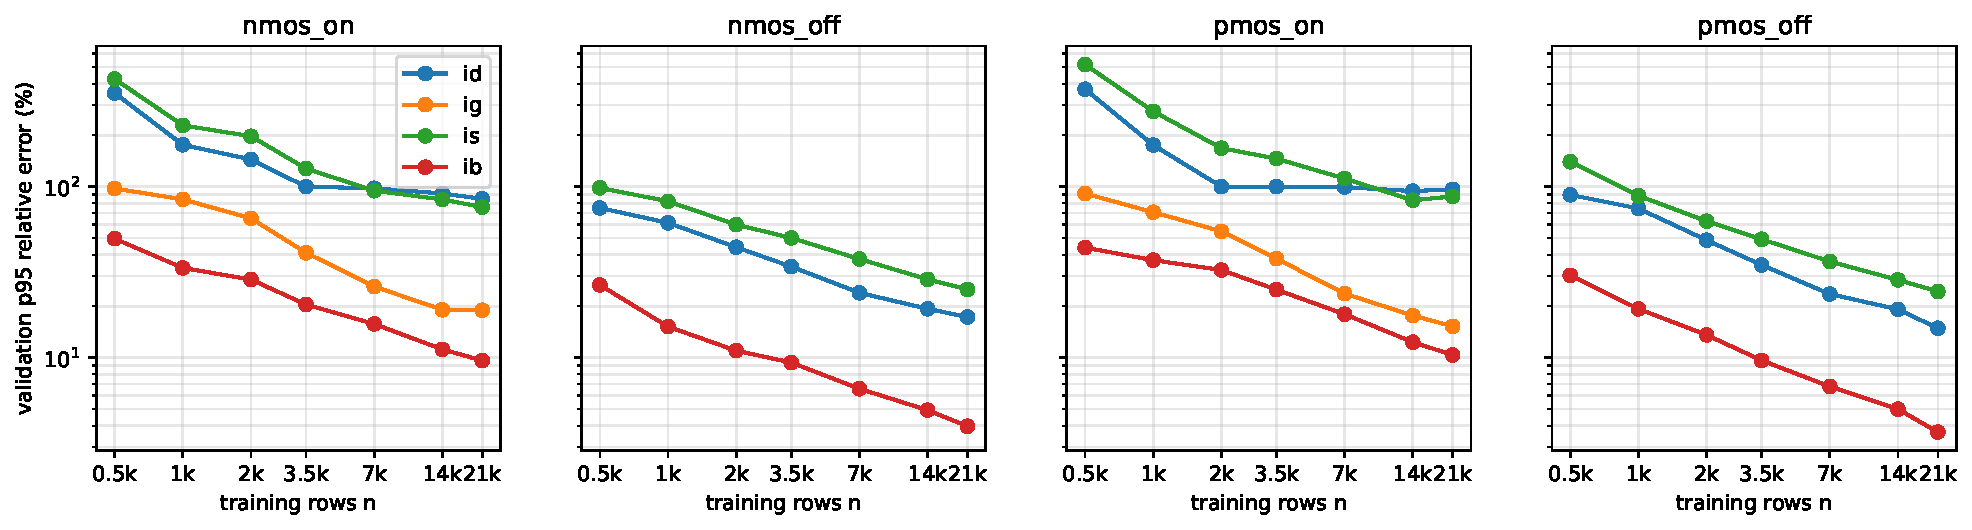
\includegraphics[width=0.85\linewidth]{learning_curve.pdf}
  \caption{Learning curve: validation p95 error of the chosen model recipe against training rows
  (log--log). Every curve still falls at \num{7000} rows. ON $I_D$/$I_S$ stay high for a different
  reason: their p95 is set by rows where the channel current crosses zero
  (Section~\ref{sec:errtrans}).}
  \label{fig:lc}
\end{figure}

\subsection{Data check}
\paragraph{Kirchhoff's law.}
The four terminal currents must sum to zero (Table~\ref{tab:kirchhoff}). For NMOS the relative
residual is at solver level (median \KirchhoffMedianRelNmosOn{} ON, \KirchhoffMedianRelNmosOff{}
OFF). For PMOS the absolute residual stays near $10^{-16}$\,A (p95 \KirchhoffPninetyfiveAbsPmosOn{}
ON, \KirchhoffPninetyfiveAbsPmosOff{} OFF), which we attribute to rounding in the body-resistance
network of \texttt{rbodymod=1}; it shows up in relative terms (up to \KirchhoffWorstRel) only
where all four currents are tiny. No row violates KCL beyond this floor, which also confirms our
sign convention.

\begin{table}[H]
  \centering
  \small
  \caption{Kirchhoff check (D3): residual $|I_D+I_G+I_S+I_B|$ over all \RowsPerCase{} rows per case.}
  \label{tab:kirchhoff}
  \fittable{% Generated by report/make_numbers.py from results/tables/kirchhoff.csv. Do not edit.
\begin{tabular}{lrrrrrr}
\toprule
 & \multicolumn{3}{c}{$|I_D+I_G+I_S+I_B|$ (A)} & \multicolumn{3}{c}{relative to $\max|I|$} \\
\cmidrule(lr){2-4}\cmidrule(lr){5-7}
Case & median & p95 & max & median & p95 & max \\
\midrule
\texttt{nmos\_on} & \num{4.0e-20} & \num{4.6e-16} & \num{9.7e-15} & \num{1.1e-11} & \num{1.4e-10} & \num{3.7e-08} \\
\texttt{nmos\_off} & \num{1.1e-24} & \num{4.8e-22} & \num{9.9e-21} & \num{1.2e-11} & \num{5.9e-11} & \num{1.1e-10} \\
\texttt{pmos\_on} & \num{3.3e-17} & \num{3.0e-16} & \num{9.1e-15} & \num{8.0e-09} & \num{3.1e-03} & \num{1.3e-02} \\
\texttt{pmos\_off} & \num{2.6e-17} & \num{7.2e-17} & \num{1.7e-16} & \num{1.5e-04} & \num{4.7e-03} & \num{8.5e-02} \\
\bottomrule
\end{tabular}
}
\end{table}

\paragraph{Trends.}
Figure~\ref{fig:trends} confirms the expected physics: the OFF current rises exponentially with
temperature and falls exponentially with $|V_{th0}|$ (subthreshold conduction), and the gate
current falls exponentially with \texttt{toxe} (tunnelling), with the ON cases many decades above
the OFF cases, where only the gate--drain overlap tunnels. The flat floor near $10^{-14}$\,A in the
OFF current is BSIM4's default junction current, since the decks give no junction areas.

\begin{figure}[H]
  \centering
  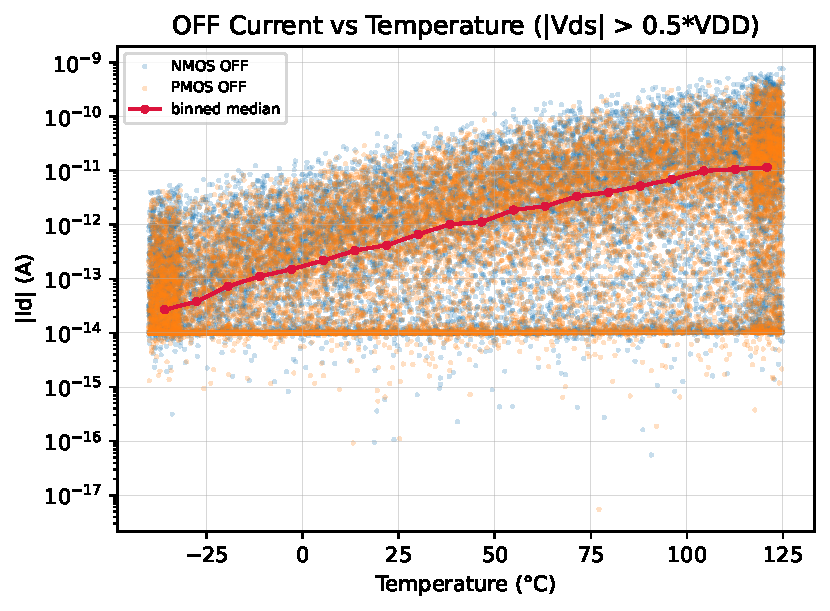
\includegraphics[width=0.32\linewidth]{trend_ioff_vs_temp.pdf}\hfill
  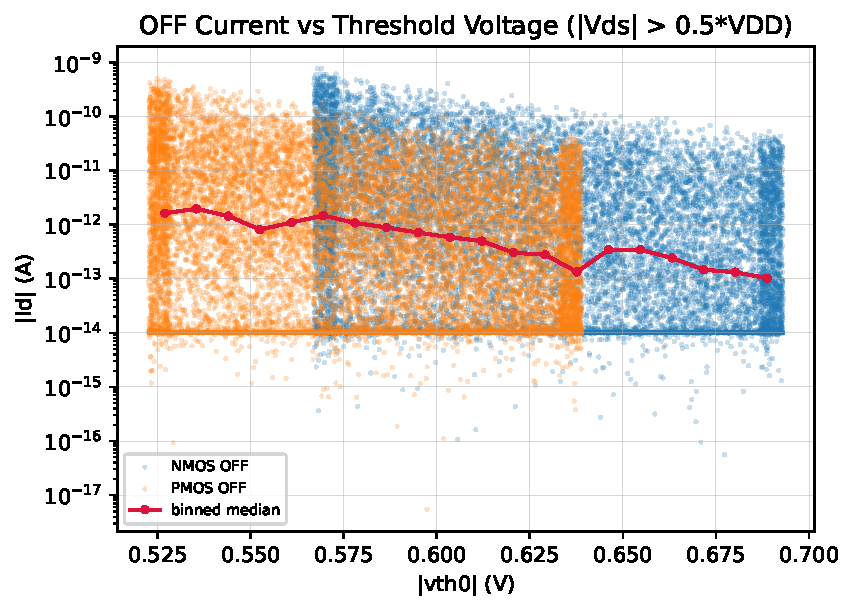
\includegraphics[width=0.32\linewidth]{trend_ioff_vs_vth0.pdf}\hfill
  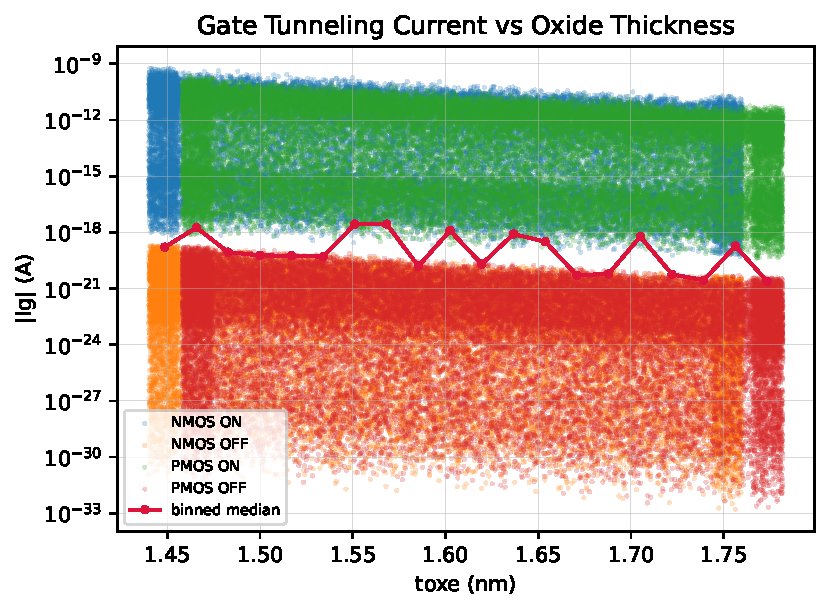
\includegraphics[width=0.32\linewidth]{trend_ig_vs_toxe.pdf}
  \caption{Data-check trends (D3): OFF drain current vs temperature (left) and vs $|V_{th0}|$
  (centre); gate current vs \texttt{toxe} for all cases (right). Dense strips at the range edges
  are the boundary rows.}
  \label{fig:trends}
\end{figure}

% Transistor models
\section{Transistor models}\label{sec:models}

\todo{four model types, hyperparameters, preprocessing, comparison table, chosen models on test}

% Gate results
\section{Gate results}\label{sec:gates}

\subsection{Setup and SPICE reference}
We evaluate INV, NAND2, NOR2 and AND2/OR2 (NAND2/NOR2 + inverter): 18 input cases, each at the
same \NumCorners{} PVT corners. A corner is one draw of $V_{DD}$, $T$ and the process parameters
(one draw for all NMOS, one for all PMOS); the corners are drawn once (seed \SeedCorners) and
reused by the test circuit. Each of the \NumGateSims{} combinations is simulated as one complete
deck (AND2/OR2 as single decks, not NAND2 + INV added), inputs at exactly $0$ or $V_{DD}$. The
leakage is the supply current $I_{VDD}=-\texttt{i(vvdd)}$; each deck also records the output and
internal nodes ($x$ between series NMOS, $y$ between series PMOS, $n_1$ at the AND2/OR2 first
stage). The output passes the logic check in \GateLogicOk{} rows.

\subsection{From transistor models to gate leakage}
For every (gate, inputs, corner) we (1) take the output and internal node voltages from SPICE, as
the brief prescribes; (2) derive each transistor's $(V_D,V_G,V_S,V_B)$, case, width and corner
parameters from the topology; (3) predict all transistors of all \NumGateSims{} rows in one
batched call; and (4) apply KCL on the VDD net: $I_{VDD}$ is the sum of the currents into all
terminals tied to VDD (PMOS sources and bodies). The same bookkeeping on the input nodes gives
$I_{in}$, the tunnelling current drawn by inputs at logic~1, which the test circuit needs. The
models only saw $V_G\in\{0,V_{DD}\}$, so the AND2/OR2 inverter gate (driven by $n_1$) is snapped to
the nearest rail; the largest snap is \GateSnapMax{}.

\subsection{Why the direct sum failed, and the KCL composition}\label{sec:kcl}
Our first implementation summed the predicted currents directly. With the first models this gave
a median error of \qty{846}{\percent} and \emph{negative} leakage in \qty{77}{\percent} of rows.
The SPICE oracle below showed the bookkeeping was correct, and an attribution traced
\qty{99.7}{\percent} of the error to one term: the channel current of the ON PMOS on the VDD net.

The reason is physical. An ON transistor in a static gate is a closed switch between two nodes at
almost the same voltage: over all gate rows, the \OnVdsCount{} such transistors have median
$|V_{DS}|$ = \OnVdsMedian{} and at most \OnVdsMax. Their channel current is set by the rest of the
gate (typically the OFF device they feed), not by their own minute $V_{DS}$, so predicting it from
$V_{DS}$ is ill-posed: even rounding these voltages to 10 digits changes the SPICE current by
\qty{0.3}{\percent}. More training data near $V_{DS}\approx 0$ fixed the sign but not the
magnitude (60--\qty{100}{\percent} error in our tests).

We therefore treat the channel current of every ON transistor with $|V_{DS}| <$ \KclVdsMax{} as
an unknown. Its predicted $I_G$ and $I_B$ are kept (they have no zero crossing), its drain current
is solved from KCL at the floating nodes (output, $x$, $y$, $n_1$), and $I_S=-(I_D+I_G+I_B)$. All
other transistors keep their model currents. The threshold lies orders of magnitude above the
in-gate ON values and below the smallest genuinely biased ON transistor (\OnBiasedVdsMin, e.g.\
the lower PMOS of NOR2 \texttt{10}), which keeps its model current. Parallel ON transistors (both
PMOS of NAND2 \texttt{00}) leave only their sum determined; we take the minimum-norm
(pseudo-inverse) solution. Any other split adds a current circulating around the parallel loop,
which enters and leaves the VDD net and cannot change $I_{VDD}$; the code checks this for every
pattern. $I_{in}$ is unaffected, since gate currents are never corrected.

\paragraph{SPICE-oracle validation.}
To test the composition independently of the ML models, we simulated every transistor of every
gate row \emph{alone} in ngspice at exactly the terminal voltages the model sees, and fed these
SPICE currents through the same composition. Over all \NumGateSims{} rows this reproduces the
gate SPICE leakage with mean accuracy \OracleMeanAcc{} (median error \OracleMedianErr, p95
\OraclePninetyfiveErr, max \OracleMaxErr). The topology mapping, signs, widths, corner parameters
and the KCL solve are therefore exact well below the ML error, and \emph{all} remaining gate error
comes from the transistor models.

\subsection{Results (D6, D7)}
Over all rows the gate leakage reaches a mean accuracy of \GateMeanAcc{}: median error
\GateMedianErr, p95 \GatePninetyfiveErr, maximum \GateMaxErr, bias \GateBias, and \GateWithinTen{}
of rows within \qty{10}{\percent} of SPICE (Table~\ref{tab:gates}, Figure~\ref{fig:gateparity}).
With the same final models the direct sum reaches only \GateDirectMeanAcc{} (median
\GateDirectMedianErr, p95 \GateDirectPninetyfiveErr): the KCL composition is still essential.

\begin{table}[H]
  \centering
  \small
  \caption{Gate results (D6), KCL composition, \NumCorners{} corners per case: SPICE and ML median
  leakage, bias (median signed error), median and p95 absolute error, mean accuracy. Last row: all
  \NumGateSims{} rows.}
  \label{tab:gates}
  \fittable{% Generated by report/make_numbers.py from results/tables/gate_results.csv. Do not edit.
\begin{tabular}{llrrrrrr}
\toprule
Gate & Inputs & SPICE median (A) & ML median (A) & Bias & Median err. & p95 err. & Mean acc. \\
\midrule
INV & \texttt{0} & \num{1.63e-11} & \num{1.64e-11} & \qty[retain-explicit-plus]{+0.17}{\percent} & \qty{0.98}{\percent} & \qty{2.93}{\percent} & \qty{98.85}{\percent} \\
 & \texttt{1} & \num{5.43e-12} & \num{5.37e-12} & \qty[retain-explicit-plus]{+0.17}{\percent} & \qty{1.34}{\percent} & \qty{4.07}{\percent} & \qty{98.45}{\percent} \\
\midrule
NAND2 & \texttt{00} & \num{1.79e-11} & \num{1.79e-11} & \qty[retain-explicit-plus]{+0.14}{\percent} & \qty{1.16}{\percent} & \qty{3.39}{\percent} & \qty{98.66}{\percent} \\
 & \texttt{01} & \num{1.63e-11} & \num{1.64e-11} & \qty[retain-explicit-plus]{+0.18}{\percent} & \qty{0.98}{\percent} & \qty{2.94}{\percent} & \qty{98.85}{\percent} \\
 & \texttt{10} & \num{1.34e-11} & \num{1.31e-11} & \qty[retain-explicit-plus]{-0.60}{\percent} & \qty{1.62}{\percent} & \qty{8.63}{\percent} & \qty{97.39}{\percent} \\
 & \texttt{11} & \num{1.09e-11} & \num{1.07e-11} & \qty[retain-explicit-plus]{+0.17}{\percent} & \qty{1.34}{\percent} & \qty{4.06}{\percent} & \qty{98.46}{\percent} \\
\midrule
NOR2 & \texttt{00} & \num{3.27e-11} & \num{3.29e-11} & \qty[retain-explicit-plus]{+0.14}{\percent} & \qty{0.96}{\percent} & \qty{2.85}{\percent} & \qty{98.86}{\percent} \\
 & \texttt{01} & \num{1.80e-11} & \num{1.81e-11} & \qty[retain-explicit-plus]{+0.33}{\percent} & \qty{1.09}{\percent} & \qty{3.09}{\percent} & \qty{98.74}{\percent} \\
 & \texttt{10} & \num{2.94e-12} & \num{2.90e-12} & \qty[retain-explicit-plus]{+0.67}{\percent} & \qty{1.95}{\percent} & \qty{7.38}{\percent} & \qty{97.30}{\percent} \\
 & \texttt{11} & \num{4.79e-13} & \num{4.71e-13} & \qty[retain-explicit-plus]{+0.49}{\percent} & \qty{2.33}{\percent} & \qty{7.53}{\percent} & \qty{97.10}{\percent} \\
\midrule
AND2 & \texttt{00} & \num{4.56e-11} & \num{4.55e-11} & \qty[retain-explicit-plus]{+0.18}{\percent} & \qty{0.91}{\percent} & \qty{2.82}{\percent} & \qty{98.89}{\percent} \\
 & \texttt{01} & \num{4.02e-11} & \num{4.05e-11} & \qty[retain-explicit-plus]{+0.01}{\percent} & \qty{0.82}{\percent} & \qty{2.50}{\percent} & \qty{98.99}{\percent} \\
 & \texttt{10} & \num{3.88e-11} & \num{3.84e-11} & \qty[retain-explicit-plus]{-0.41}{\percent} & \qty{1.16}{\percent} & \qty{4.03}{\percent} & \qty{98.59}{\percent} \\
 & \texttt{11} & \num{3.44e-11} & \num{3.45e-11} & \qty[retain-explicit-plus]{+0.28}{\percent} & \qty{0.98}{\percent} & \qty{2.62}{\percent} & \qty{98.89}{\percent} \\
\midrule
OR2 & \texttt{00} & \num{5.91e-11} & \num{5.96e-11} & \qty[retain-explicit-plus]{+0.09}{\percent} & \qty{0.84}{\percent} & \qty{2.42}{\percent} & \qty{99.00}{\percent} \\
 & \texttt{01} & \num{3.49e-11} & \num{3.49e-11} & \qty[retain-explicit-plus]{+0.27}{\percent} & \qty{1.04}{\percent} & \qty{2.85}{\percent} & \qty{98.86}{\percent} \\
 & \texttt{10} & \num{2.23e-11} & \num{2.26e-11} & \qty[retain-explicit-plus]{+0.36}{\percent} & \qty{1.05}{\percent} & \qty{3.21}{\percent} & \qty{98.80}{\percent} \\
 & \texttt{11} & \num{1.80e-11} & \num{1.79e-11} & \qty[retain-explicit-plus]{+0.19}{\percent} & \qty{0.95}{\percent} & \qty{2.80}{\percent} & \qty{98.90}{\percent} \\
\midrule
\textbf{All} &  & \num{2.01e-11} & \num{2.02e-11} & \qty[retain-explicit-plus]{+0.15}{\percent} & \qty{1.13}{\percent} & \qty{4.13}{\percent} & \qty{98.53}{\percent} \\
\bottomrule
\end{tabular}
}
\end{table}

\begin{figure}[H]
  \centering
  \begin{minipage}[t]{0.49\linewidth}
    \centering
    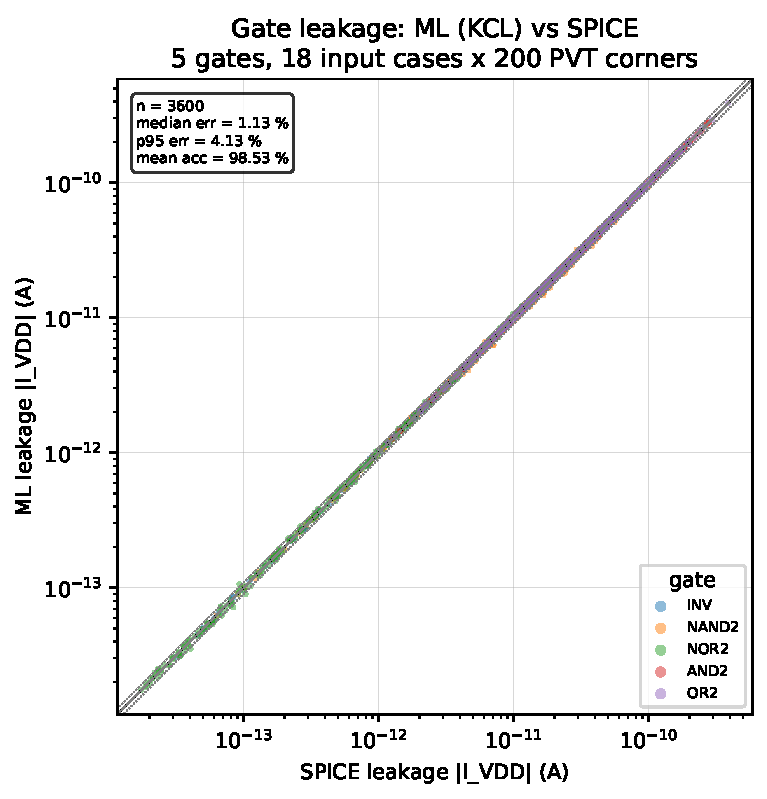
\includegraphics[width=\linewidth]{gate_parity.pdf}
    \caption{Gate parity plot (D7), KCL composition, all \NumGateSims{} rows.}
    \label{fig:gateparity}
  \end{minipage}\hfill
  \begin{minipage}[t]{0.49\linewidth}
    \centering
    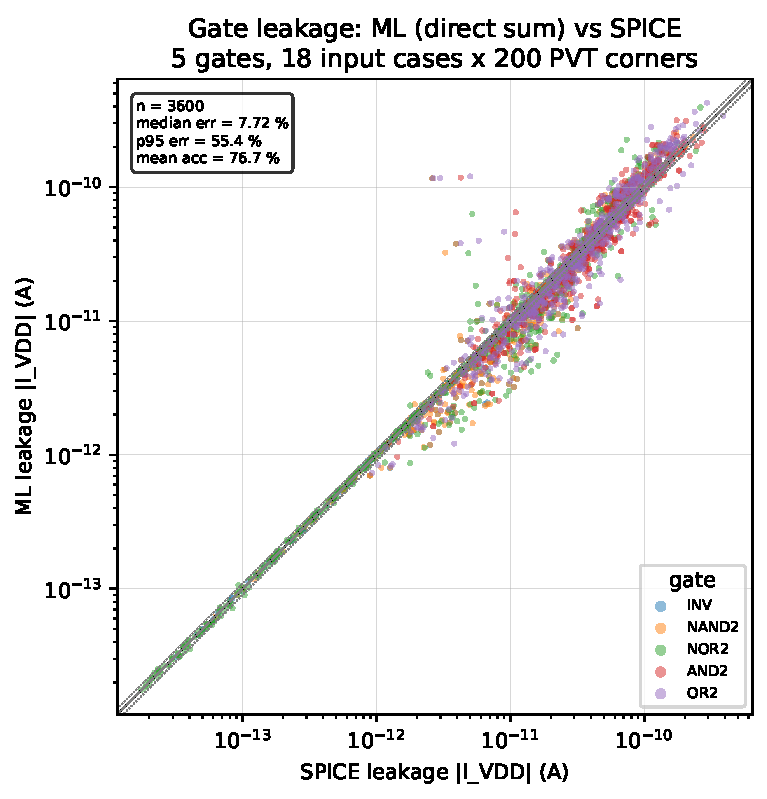
\includegraphics[width=\linewidth]{gate_parity_direct.pdf}
    \caption{Direct sum with the same models. Cases without an ON PMOS on the VDD net agree;
    the others scatter.}
    \label{fig:gateparitydirect}
  \end{minipage}
\end{figure}

\paragraph{Most and least accurate cases.}
The most accurate case is \GateBestCase{} (\GateBestAcc): its leakage is set by OFF transistors at
the full-$V_{DD}$ OFF point that source and drain pinning oversample, while all its ON transistors
are handled by KCL. The least accurate is \GateWorstCase{} (\GateWorstAcc). NAND2 \texttt{10} was the weakest
case for most of the project: its upper NMOS is ON but can only pull $x$ to about a threshold
below $V_{DD}$, so it conducts at a substantial $|V_{DS}|$, is not KCL-corrected, and its predicted
drain current enters the output-node KCL. Before stack pinning, replacing only that current with its SPICE
value raised the case from \qty{94.8}{\percent} to \qty{97.6}{\percent}, which is why we added
stack pinning (Section~\ref{sec:oversampling}); it lifted NAND2 \texttt{10} to \GateNandTenAcc. The
worst individual rows are listed in Table~\ref{tab:gateworst}.

\begin{table}[H]
  \centering
  \small
  \caption{Gate rows with the largest relative error.}
  \label{tab:gateworst}
  \fittable{% Generated by report/make_numbers.py from results/tables/gate_worst_cases.csv. Do not edit.
\begin{tabular}{llrrrrrr}
\toprule
Gate & Inputs & Corner & $T$ (\si{\degreeCelsius}) & $V_{DD}$ (V) & SPICE (A) & ML (A) & Error \\
\midrule
NOR2 & \texttt{10} & 4 & \num{-27.8} & \num{0.980} & \num{8.39e-14} & \num{7.16e-14} & \qty[retain-explicit-plus]{-14.7}{\percent} \\
NOR2 & \texttt{11} & 151 & \num{21.1} & \num{0.852} & \num{9.30e-14} & \num{1.07e-13} & \qty[retain-explicit-plus]{+14.6}{\percent} \\
NOR2 & \texttt{10} & 95 & \num{-26.0} & \num{0.859} & \num{1.03e-13} & \num{8.97e-14} & \qty[retain-explicit-plus]{-13.0}{\percent} \\
NOR2 & \texttt{11} & 195 & \num{9.1} & \num{0.858} & \num{4.03e-14} & \num{3.54e-14} & \qty[retain-explicit-plus]{-12.3}{\percent} \\
NAND2 & \texttt{10} & 25 & \num{53.4} & \num{0.850} & \num{1.66e-11} & \num{1.47e-11} & \qty[retain-explicit-plus]{-11.7}{\percent} \\
NAND2 & \texttt{10} & 186 & \num{69.9} & \num{0.821} & \num{7.08e-12} & \num{6.26e-12} & \qty[retain-explicit-plus]{-11.6}{\percent} \\
NAND2 & \texttt{10} & 119 & \num{99.8} & \num{0.838} & \num{4.61e-12} & \num{4.09e-12} & \qty[retain-explicit-plus]{-11.3}{\percent} \\
NAND2 & \texttt{10} & 184 & \num{123.1} & \num{0.961} & \num{3.82e-11} & \num{3.41e-11} & \qty[retain-explicit-plus]{-10.7}{\percent} \\
NAND2 & \texttt{10} & 64 & \num{64.7} & \num{0.846} & \num{7.02e-12} & \num{6.29e-12} & \qty[retain-explicit-plus]{-10.4}{\percent} \\
NAND2 & \texttt{10} & 145 & \num{43.5} & \num{0.892} & \num{1.87e-11} & \num{1.68e-11} & \qty[retain-explicit-plus]{-10.2}{\percent} \\
NAND2 & \texttt{10} & 65 & \num{92.1} & \num{0.895} & \num{2.39e-11} & \num{2.15e-11} & \qty[retain-explicit-plus]{-10.2}{\percent} \\
NOR2 & \texttt{10} & 87 & \num{-28.5} & \num{0.832} & \num{6.89e-14} & \num{6.22e-14} & \qty[retain-explicit-plus]{-9.7}{\percent} \\
NAND2 & \texttt{10} & 50 & \num{109.0} & \num{0.943} & \num{2.92e-11} & \num{3.19e-11} & \qty[retain-explicit-plus]{+9.3}{\percent} \\
NOR2 & \texttt{11} & 120 & \num{13.4} & \num{0.859} & \num{6.71e-13} & \num{6.10e-13} & \qty[retain-explicit-plus]{-9.1}{\percent} \\
NOR2 & \texttt{10} & 150 & \num{-31.4} & \num{0.976} & \num{1.12e-13} & \num{1.02e-13} & \qty[retain-explicit-plus]{-8.9}{\percent} \\
NOR2 & \texttt{11} & 144 & \num{15.8} & \num{0.921} & \num{2.62e-13} & \num{2.85e-13} & \qty[retain-explicit-plus]{+8.8}{\percent} \\
NAND2 & \texttt{10} & 115 & \num{120.7} & \num{0.851} & \num{2.69e-11} & \num{2.45e-11} & \qty[retain-explicit-plus]{-8.8}{\percent} \\
NOR2 & \texttt{11} & 109 & \num{47.7} & \num{0.838} & \num{4.78e-13} & \num{4.36e-13} & \qty[retain-explicit-plus]{-8.7}{\percent} \\
NAND2 & \texttt{10} & 161 & \num{122.7} & \num{0.853} & \num{1.68e-11} & \num{1.54e-11} & \qty[retain-explicit-plus]{-8.6}{\percent} \\
NAND2 & \texttt{10} & 154 & \num{70.3} & \num{0.824} & \num{4.19e-12} & \num{3.83e-12} & \qty[retain-explicit-plus]{-8.6}{\percent} \\
\bottomrule
\end{tabular}
}
\end{table}

\paragraph{Input current.}
$I_{in}$ is predicted with mean accuracy \GateIinMeanAcc{} (median \GateIinMedianErr, p95
\GateIinPninetyfiveErr, bias \GateIinBias). It is far from negligible: in rows with a high input
it is \GateIinShare{} of $I_{VDD}$ at the median, which matters for the test circuit.

\subsection{How the accuracy developed}\label{sec:history}
Table~\ref{tab:history} summarises our iterations. The large steps came from the composition and
from sampling the right operating points; the model change that mattered was the linear leaves.

\begin{table}[H]
  \centering
  \small
  \caption{Development of the gate-level accuracy (18 cases, \NumCorners{} corners). Rows 1--3
  and 5: earlier runs as recorded; rows 4 and 6: generated.}
  \label{tab:history}
  \begin{tabular}{@{}>{\raggedright\arraybackslash}p{0.52\linewidth}lrr@{}}
    \toprule
    Stage & Composition & Median err. & Mean acc. \\
    \midrule
    1.\ first models, uniform data & direct & \qty{846}{\percent} & -- \\
    2.\ + low-$|V_{DS}|$ ON rows & direct & \qty{14}{\percent} & -- \\
    3.\ + KCL composition & KCL & \qty{7.0}{\percent} & \qty{91.5}{\percent} \\
    4.\ \RowsPerCase{} rows, source and drain pinning, constant leaves & KCL &
        \ConstLeafGateMedianErr & \ConstLeafGateMeanAcc \\
    5.\ + linear-leaf GBDT & KCL & -- & \qty{97.6}{\percent} \\
    6.\ final: + ON stack pinning & KCL & \GateMedianErr & \GateMeanAcc \\
    \bottomrule
  \end{tabular}
\end{table}

\subsection{Generalisation to fresh corners}\label{sec:fresh}
Because the sampling rules were guided by gate errors on the \NumCorners{} evaluation corners, we
repeated the full gate evaluation on \FreshNumCorners{} \emph{new} corners (seed \FreshSeed),
with new SPICE references (logic check \FreshLogicOk) and unchanged models. There is no
degradation (Table~\ref{tab:fresh}): \FreshMeanAcc{} mean accuracy (median \FreshMedianErr, p95
\FreshPninetyfiveErr) against \GateMeanAcc{} on the original corners.

\begin{table}[H]
  \centering
  \small
  \caption{Gate accuracy on the evaluation corners and on \FreshNumCorners{} fresh corners.}
  \label{tab:fresh}
  \fittable{% Generated by report/make_numbers.py from report/analysis/fresh_corners/overall_kcl_direct_orig_vs_fresh.csv. Do not edit.
\begin{tabular}{llrrrrr}
\toprule
Corners & Composition & Median err. & p95 err. & Max err. & Bias & Mean acc. \\
\midrule
original & KCL & \qty{1.82}{\percent} & \qty{6.20}{\percent} & \qty{26.4}{\percent} & \qty[retain-explicit-plus]{+1.04}{\percent} & \qty{97.61}{\percent} \\
 & direct & \qty{7.47}{\percent} & \qty{55.30}{\percent} & \qty{2567.4}{\percent} & \qty[retain-explicit-plus]{-2.02}{\percent} & \qty{79.63}{\percent} \\
\midrule
fresh & KCL & \qty{1.70}{\percent} & \qty{5.93}{\percent} & \qty{29.2}{\percent} & \qty[retain-explicit-plus]{+0.70}{\percent} & \qty{97.69}{\percent} \\
 & direct & \qty{6.92}{\percent} & \qty{52.97}{\percent} & \qty{628.5}{\percent} & \qty[retain-explicit-plus]{-2.19}{\percent} & \qty{83.30}{\percent} \\
\bottomrule
\end{tabular}
}
\end{table}

% Test circuit
\section{Test-circuit results}\label{sec:circuit}

\subsection{Circuit and SPICE reference}
The \TestCircuit{} computes the XOR of \CircuitNumInputs{} inputs with a balanced tree of
\CircuitNumXor{} XOR2 gates. Since only the Part~B gates have leakage models, each XOR2 is built
from four NAND2 ($n_1=\overline{ab}$, $n_2=\overline{a n_1}$, $n_3=\overline{b n_1}$,
$\mathit{out}=\overline{n_2 n_3}$), giving \CircuitGateMix{} gates. All \CircuitNumVectors{}
vectors are evaluated at the same \NumCorners{} corners as the gates (\CircuitNumSims{} cases). The
SPICE reference is one flat transistor-level deck per (vector, corner), with the same subcircuits,
sizing and corners; internal nets are driven by real gates, so loading is physically present. The
output is correct in \CircuitLogicOk{} decks.

\subsection{Hierarchical ML prediction and the loading term}
A logic simulation gives every gate instance its input bits; each instance's leakage is the
Part~B ML result for that gate, input combination and corner. No SPICE quantity of the circuit is
used.

The plain gate sum under-estimated the circuit by \CircuitNoLoadBias{} (median, mean accuracy
\CircuitNoLoadMeanAcc), far more than the gate errors could explain. The missing current is
physical: in Part~B a gate's inputs are ideal sources, so the tunnelling current drawn by a high
input ($I_{in}$) is not in that gate's $I_{VDD}$. In the circuit, a high internal net is held up
by the ON PMOS of its driver, so the same current is drawn from VDD (a low net sinks into the
driver's pull-down and adds nothing). We therefore add a loading term:
\begin{equation}
  I_{VDD}^{ML} = \sum_{\text{gates}} I_{VDD}^{ML}(\text{gate},\text{bits})
  + \sum_{\text{gates}} f_{\text{int}}\, I_{in}^{ML}(\text{gate},\text{bits}),
\end{equation}
where $f_{\text{int}}$ is the share of the gate's high input pins driven by another gate (pins fed
by primary inputs draw from the testbench sources, as in the SPICE deck). On this low-power card
the term is large: it is \CircuitLoadShare{} of the predicted circuit leakage (median).

To separate the composition from the ML error, we also composed the circuit from the Part~B
\emph{SPICE} gate values with the same loading term. This reproduces the circuit SPICE leakage with
mean accuracy \CompSpiceMeanAcc{} (max error \CompSpiceMaxErr), so the hierarchical composition and
the loading term are essentially exact for this circuit, and the circuit error is inherited
entirely from the gate-level ML error.

\subsection{Results (D8)}
Over all \CircuitNumSims{} cases the mean accuracy is \CircuitMeanAcc: median error
\CircuitMedianErr, p95 \CircuitPninetyfiveErr, maximum \CircuitMaxErr, bias \CircuitBias{}
(Table~\ref{tab:circuit}, Figure~\ref{fig:circuitparity}). Grouped by the number of ones in the
vector, the accuracy stays between \CircuitOnesAccMin{} and \CircuitOnesAccMax.

\begin{table}[H]
  \centering
  \small
  \caption{Test-circuit results (D8): all vectors, then by number of ones. Below the rule: without
  the loading term, the primary-input current, and the gate-level result for comparison.}
  \label{tab:circuit}
  \fittable{% Generated by report/make_numbers.py from results/tables/circuit_results.csv. Do not edit.
\begin{tabular}{lrrrrrrrr}
\toprule
Scope & $n$ & SPICE median (A) & ML median (A) & Bias & Median err. & p95 err. & Max err. & Mean acc. \\
\midrule
all vectors & \num{51200} & \num{8.04e-10} & \num{8.11e-10} & \qty[retain-explicit-plus]{-0.16}{\percent} & \qty{0.92}{\percent} & \qty{2.91}{\percent} & \qty{5.1}{\percent} & \qty{98.92}{\percent} \\
\midrule
\quad 0 ones & \num{200} & \num{9.00e-10} & \num{9.02e-10} & \qty[retain-explicit-plus]{+0.04}{\percent} & \qty{0.87}{\percent} & \qty{2.68}{\percent} & \qty{5.1}{\percent} & \qty{98.96}{\percent} \\
\quad 1 ones & \num{1600} & \num{8.77e-10} & \num{8.75e-10} & \qty[retain-explicit-plus]{-0.03}{\percent} & \qty{0.84}{\percent} & \qty{2.73}{\percent} & \qty{5.1}{\percent} & \qty{98.96}{\percent} \\
\quad 2 ones & \num{5600} & \num{8.63e-10} & \num{8.66e-10} & \qty[retain-explicit-plus]{-0.10}{\percent} & \qty{0.88}{\percent} & \qty{2.81}{\percent} & \qty{5.1}{\percent} & \qty{98.94}{\percent} \\
\quad 3 ones & \num{11200} & \num{8.34e-10} & \num{8.39e-10} & \qty[retain-explicit-plus]{-0.14}{\percent} & \qty{0.91}{\percent} & \qty{2.88}{\percent} & \qty{5.1}{\percent} & \qty{98.93}{\percent} \\
\quad 4 ones & \num{14000} & \num{8.05e-10} & \num{8.13e-10} & \qty[retain-explicit-plus]{-0.15}{\percent} & \qty{0.93}{\percent} & \qty{2.94}{\percent} & \qty{5.0}{\percent} & \qty{98.92}{\percent} \\
\quad 5 ones & \num{11200} & \num{7.77e-10} & \num{7.84e-10} & \qty[retain-explicit-plus]{-0.20}{\percent} & \qty{0.97}{\percent} & \qty{2.97}{\percent} & \qty{5.0}{\percent} & \qty{98.91}{\percent} \\
\quad 6 ones & \num{5600} & \num{7.78e-10} & \num{7.74e-10} & \qty[retain-explicit-plus]{-0.22}{\percent} & \qty{0.98}{\percent} & \qty{2.99}{\percent} & \qty{4.9}{\percent} & \qty{98.89}{\percent} \\
\quad 7 ones & \num{1600} & \num{7.61e-10} & \num{7.66e-10} & \qty[retain-explicit-plus]{-0.21}{\percent} & \qty{0.97}{\percent} & \qty{3.04}{\percent} & \qty{4.8}{\percent} & \qty{98.89}{\percent} \\
\quad 8 ones & \num{200} & \num{7.90e-10} & \num{7.82e-10} & \qty[retain-explicit-plus]{-0.19}{\percent} & \qty{0.93}{\percent} & \qty{3.01}{\percent} & \qty{4.6}{\percent} & \qty{98.89}{\percent} \\
\midrule
without loading term & \num{51200} & \num{8.04e-10} & \num{4.82e-10} & \qty[retain-explicit-plus]{-27.59}{\percent} & \qty{27.59}{\percent} & \qty{81.70}{\percent} & \qty{96.0}{\percent} & \qty{64.79}{\percent} \\
primary-input current $I_{in}$ & \num{51200} & \num{3.43e-11} & \num{3.44e-11} & \qty[retain-explicit-plus]{-0.71}{\percent} & \qty{1.43}{\percent} & \qty{4.14}{\percent} & \qty{6.7}{\percent} & \qty{98.34}{\percent} \\
gate level (all gates) & \num{3600} & \num{2.01e-11} & \num{2.02e-11} & \qty[retain-explicit-plus]{+0.15}{\percent} & \qty{1.13}{\percent} & \qty{4.13}{\percent} & \qty{14.7}{\percent} & \qty{98.53}{\percent} \\
\bottomrule
\end{tabular}
}
\end{table}

\begin{figure}[H]
  \centering
  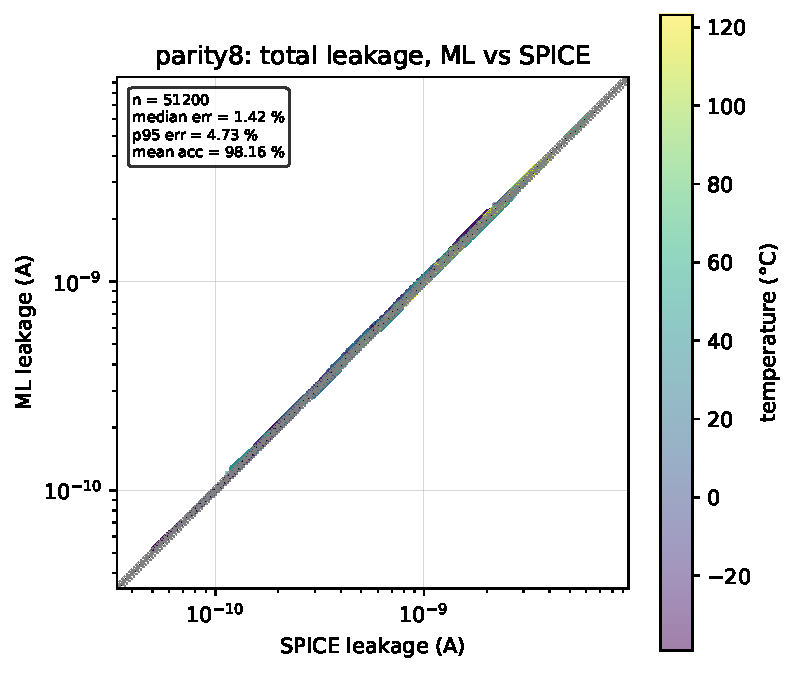
\includegraphics[width=0.6\linewidth]{circuit_parity.pdf}
  \caption{Circuit parity plot (D8), all \CircuitNumSims{} cases, coloured by temperature. The
  coldest corners sit slightly above the diagonal (Section~\ref{sec:errcircuit}).}
  \label{fig:circuitparity}
\end{figure}

\paragraph{Circuit versus gate accuracy.}
The brief expects the circuit to be less accurate than the gates. With the loading term it is
slightly \emph{more} accurate: \CircuitMeanAcc{} against \GateNandMeanAcc{} over the NAND2 cases
(its only gate type), with much smaller tails (p95 \CircuitPninetyfiveErr{} vs
\GateNandPninetyfiveErr, max \CircuitMaxErr{} vs \GateNandMaxErr). The circuit leakage is a sum
over \CircuitNumGates{} instances in different input states, so the instance-to-instance part of
the gate error partly cancels. The cancellation is incomplete because all instances share one
corner, and a systematic bias does not cancel at all: the circuit bias (\CircuitBias) stays of the
order of the NAND2 bias (\GateNandBias). The circuit accuracy is therefore limited by the
systematic part of the transistor-model error, not by its scatter.

% Error analysis
\section{Error analysis}\label{sec:error}

\todo{largest errors by case, gate, input combination and corner conditions, and why}

% Limitations and improvements
\section{Limitations and improvements}\label{sec:limitations}

\paragraph{Final accuracy against the target.}
The brief sets a target of up to \qty{99}{\percent} mean accuracy. We reach \GateMeanAcc{} at gate
level, \FreshMeanAcc{} on fresh corners, and \CircuitMeanAcc{} on the test circuit, so the target
is not met, by about one to two percentage points. The analysis of Section~\ref{sec:error} locates
the gap precisely: the composition is exact (SPICE oracle \OracleMeanAcc, circuit composition from
SPICE gate values \CompSpiceMeanAcc), so all of the remaining error comes from the transistor models,
and the single largest contribution, \ErrorSourceFirst{}, would on its own raise the gate accuracy
to \ErrorSourceFirstAcc{} if it were exact. The limitations below are grouped by part, each with
the change we would make.

\begin{itemize}
  \item \textbf{Data and sampling}
  \begin{itemize}
    \item \emph{ON transistors at intermediate $|V_{DS}|$.} The sampling targets ON transistors at
          $V_{DS}\approx 0$ and OFF transistors at the rails, but an ON NMOS whose source floats at
          an internal node (the upper NMOS of NAND2~\texttt{10}, $x \approx
          \VxOneZeroFrac\,V_{DD}$) sits at a substantial $|V_{DS}|$ near threshold and causes the
          worst gate case. \emph{Improvement:} an ON-case analogue of source pinning, with the
          source drawn near $V_{DD} - V_{th}$ (NMOS) or $V_{th}$ (PMOS) and the drain on the rail;
          like the existing rules it follows from circuit physics, not from evaluation data.
    \item \emph{Dataset size.} The learning curve (Figure~\ref{fig:lc}) still slopes down at
          \LCMaxSize{} training rows. \emph{Improvement:} more rows, concentrated in the
          oversampled regions where the error is largest.
    \item \emph{Junction current floor.} The OFF currents sit on a constant floor of about
          $10^{-14}$\,A at low temperature (Figure~\ref{fig:trends}), consistent with BSIM4's
          default junction current when the netlist gives no junction areas, so junction leakage
          does not scale with $W$. \emph{Improvement:} give every transistor \texttt{AS}/\texttt{AD}
          and \texttt{PS}/\texttt{PD} from its width in all decks.
  \end{itemize}
  \item \textbf{Transistor models}
  \begin{itemize}
    \item \emph{PMOS gate tunnelling.} The largest error source at gate level is the ON PMOS gate
          current (Table~\ref{tab:errorsources}), whose error depends on the oxide thickness and
          does not average out over a corner. \emph{Improvement:} a dedicated model for $I_G$ with
          the physical $\exp(-\alpha\, t_{ox})$ dependence built into the features or the target.
    \item \emph{Accuracy floor at tiny currents.} Currents that cross zero (ON $I_D$, $I_S$) or are
          close to the \IFloor{} floor (OFF $I_S$) have unbounded relative error, and below about
          $10^{-14}$\,A even the SPICE reference is only good to a per cent or two
          (\SpiceFloorRel{} of the smallest gate leakage). \emph{Improvement:} train on the
          quantities that enter $I_{VDD}$ (the supply-side terminal currents) with a loss weighted
          by their share of the gate leakage, instead of on each terminal current separately.
    \item \emph{Grid edge and model size.} All four chosen GBDTs use the largest number of leaves
          in the grid (\ChosenHyperNmosOff), so larger trees may still help, and the linear-leaf
          models are large files. \emph{Improvement:} extend the grid, then prune or distil the
          final models.
  \end{itemize}
  \item \textbf{Gates}
  \begin{itemize}
    \item \emph{SPICE node voltages are still required.} As the brief prescribes, the gate
          prediction reads the internal and output node voltages from SPICE, so it is not yet a
          SPICE-free leakage estimator; the optional ML node solve was not implemented.
          \emph{Improvement:} solve KCL at the internal nodes with the ML currents (a 1-D root
          search per node, coupled for AND2/OR2) and compare the solved voltages with SPICE.
    \item \emph{Heuristic KCL threshold.} ON transistors below \KclVdsMax{} get their channel
          current from KCL. This works because the gap is wide (in-gate values at most \OnVdsMax,
          the smallest genuinely biased ON transistor at \OnBiasedVdsMin), but a gate with an
          intermediate $|V_{DS}|$ would fall between the two regimes. \emph{Improvement:} solve the
          channel currents of all ON transistors consistently with the node voltages, which the
          ML node solve above would provide.
    \item \emph{Ideal gate voltages.} The models only know $V_G\in\{0, V_{DD}\}$; the AND2/OR2
          inverter input is snapped (at most \GateSnapMax{} here). In circuits with degraded logic
          levels this would no longer be negligible. \emph{Improvement:} sample $V_G$ in a narrow
          band around each rail.
  \end{itemize}
  \item \textbf{Test circuit}
  \begin{itemize}
    \item \emph{Loading term.} The loading term assumes ideal $0$/$V_{DD}$ gate inputs and splits a
          gate's $I_{in}$ evenly over its high pins. For the NAND2-only parity checker this is
          essentially exact (\CompSpiceMeanAcc{} with SPICE gate values), but for gates with
          asymmetric inputs, such as the AND2/OR2 first stage, the even split is an approximation.
          \emph{Improvement:} predict $I_{in}$ per input pin in the gate model.
    \item \emph{Systematic error accumulates.} Corner-dependent model errors are common to all
          gates of a corner and add up in the circuit (Section~\ref{sec:errcircuit}), so the
          circuit accuracy is bounded by the systematic part of the gate error. \emph{Improvement:}
          the transistor-model improvements above; a larger circuit would not average this error
          away.
  \end{itemize}
\end{itemize}


\appendix
% Appendix
\section{Appendix}\label{sec:appendix}

\todo{example netlists (D2), reproduction commands (D9), extra tables}

\subsection{Per-current model comparison}
\begin{table}[H]
  \centering
  \scriptsize
  \setlength{\tabcolsep}{3pt}
  \caption{Model comparison on the validation set per current (Deliverable~4, full form):
  $R^2$ on $\log_{10}|I|$, median and 95th-percentile relative error. ``--'': no rows above
  \IFloor{} (OFF-state $I_G$).}
  \label{tab:modelsfull}
  \fittable{% Generated by report/make_numbers.py from results/tables/model_comparison.csv (validation, per target). Do not edit.
\begin{tabular}{llrrrrrrrrrrrr}
\toprule
 & & \multicolumn{3}{c}{$I_D$} & \multicolumn{3}{c}{$I_G$} & \multicolumn{3}{c}{$I_S$} & \multicolumn{3}{c}{$I_B$} \\
\cmidrule(lr){3-5}\cmidrule(lr){6-8}\cmidrule(lr){9-11}\cmidrule(lr){12-14}
Case & Model & $R^2$ & med. & p95 & $R^2$ & med. & p95 & $R^2$ & med. & p95 & $R^2$ & med. & p95 \\
\midrule
\texttt{nmos\_on} & Polynomial ridge & \num{0.696} & \qty{86.9}{\percent} & \qty{240}{\percent} & \num{0.826} & \qty{71.9}{\percent} & \qty{605}{\percent} & \num{0.503} & \qty{84.9}{\percent} & \qty{302}{\percent} & \num{0.981} & \qty{15.5}{\percent} & \qty{47}{\percent} \\
 & Random forest & \num{0.691} & \qty{26.6}{\percent} & \qty{100}{\percent} & \num{0.976} & \qty{25.2}{\percent} & \qty{91}{\percent} & \num{0.536} & \qty{27.7}{\percent} & \qty{100}{\percent} & \num{0.974} & \qty{11.0}{\percent} & \qty{60}{\percent} \\
 & GBDT & \num{0.967} & \qty{8.9}{\percent} & \qty{85}{\percent} & \num{0.999} & \qty{2.8}{\percent} & \qty{19}{\percent} & \num{0.996} & \qty{7.7}{\percent} & \qty{76}{\percent} & \num{0.999} & \qty{0.8}{\percent} & \qty{10}{\percent} \\
 & MLP & \num{0.651} & \qty{67.3}{\percent} & \qty{101}{\percent} & \num{0.991} & \qty{20.4}{\percent} & \qty{68}{\percent} & \num{0.503} & \qty{65.3}{\percent} & \qty{118}{\percent} & \num{0.991} & \qty{9.2}{\percent} & \qty{28}{\percent} \\
\midrule
\texttt{nmos\_off} & Polynomial ridge & \num{0.963} & \qty{19.1}{\percent} & \qty{120}{\percent} & -- & -- & -- & \num{0.956} & \qty{17.3}{\percent} & \qty{215}{\percent} & \num{0.910} & \qty{12.9}{\percent} & \qty{115}{\percent} \\
 & Random forest & \num{0.981} & \qty{8.9}{\percent} & \qty{84}{\percent} & -- & -- & -- & \num{0.842} & \qty{21.4}{\percent} & \qty{100}{\percent} & \num{0.992} & \qty{0.6}{\percent} & \qty{32}{\percent} \\
 & GBDT & \num{0.997} & \qty{1.1}{\percent} & \qty{17}{\percent} & -- & -- & -- & \num{0.995} & \qty{2.1}{\percent} & \qty{25}{\percent} & \num{1.000} & \qty{0.1}{\percent} & \qty{4}{\percent} \\
 & MLP & \num{0.995} & \qty{5.5}{\percent} & \qty{26}{\percent} & -- & -- & -- & \num{0.988} & \qty{6.7}{\percent} & \qty{45}{\percent} & \num{0.980} & \qty{4.7}{\percent} & \qty{46}{\percent} \\
\midrule
\texttt{pmos\_on} & Polynomial ridge & \num{0.653} & \qty{91.2}{\percent} & \qty{285}{\percent} & \num{0.804} & \qty{72.1}{\percent} & \qty{513}{\percent} & \num{0.391} & \qty{89.7}{\percent} & \qty{340}{\percent} & \num{0.982} & \qty{15.0}{\percent} & \qty{47}{\percent} \\
 & Random forest & \num{0.600} & \qty{26.3}{\percent} & \qty{100}{\percent} & \num{0.973} & \qty{25.2}{\percent} & \qty{90}{\percent} & \num{0.392} & \qty{27.1}{\percent} & \qty{100}{\percent} & \num{0.972} & \qty{11.4}{\percent} & \qty{66}{\percent} \\
 & GBDT & \num{0.957} & \qty{8.9}{\percent} & \qty{97}{\percent} & \num{0.999} & \qty{2.5}{\percent} & \qty{15}{\percent} & \num{0.997} & \qty{7.6}{\percent} & \qty{88}{\percent} & \num{0.998} & \qty{0.8}{\percent} & \qty{10}{\percent} \\
 & MLP & \num{0.645} & \qty{58.6}{\percent} & \qty{102}{\percent} & \num{0.986} & \qty{21.8}{\percent} & \qty{65}{\percent} & \num{0.442} & \qty{73.9}{\percent} & \qty{174}{\percent} & \num{0.991} & \qty{7.8}{\percent} & \qty{32}{\percent} \\
\midrule
\texttt{pmos\_off} & Polynomial ridge & \num{0.966} & \qty{17.0}{\percent} & \qty{106}{\percent} & -- & -- & -- & \num{0.956} & \qty{16.5}{\percent} & \qty{216}{\percent} & \num{0.915} & \qty{10.8}{\percent} & \qty{125}{\percent} \\
 & Random forest & \num{0.980} & \qty{8.1}{\percent} & \qty{79}{\percent} & -- & -- & -- & \num{0.789} & \qty{20.2}{\percent} & \qty{100}{\percent} & \num{0.992} & \qty{0.7}{\percent} & \qty{30}{\percent} \\
 & GBDT & \num{0.996} & \qty{1.1}{\percent} & \qty{15}{\percent} & -- & -- & -- & \num{0.994} & \qty{2.1}{\percent} & \qty{24}{\percent} & \num{1.000} & \qty{0.4}{\percent} & \qty{4}{\percent} \\
 & MLP & \num{0.995} & \qty{6.4}{\percent} & \qty{28}{\percent} & -- & -- & -- & \num{0.989} & \qty{9.8}{\percent} & \qty{44}{\percent} & \num{0.967} & \qty{7.9}{\percent} & \qty{43}{\percent} \\
\bottomrule
\end{tabular}
}
\end{table}


\end{document}
